\documentclass[10pt,a4paper]{memoir}

\usepackage[utf8]{inputenc}
\usepackage[english]{babel}
\usepackage{amsmath}
\usepackage{amsfonts}
\usepackage{amssymb}
\usepackage{lipsum}
\usepackage{subcaption}
\usepackage{float}
\usepackage[colorlinks]{hyperref}
\usepackage[nolist,nohyperlinks]{acronym} 
\usepackage{nameref}
\usepackage{cleveref}

\usepackage{tikz}
\usetikzlibrary{shapes,arrows,calc,positioning}
%\usepackage[margin=0.5in]{geometry}


\usepackage[color]{changebar}
\usepackage{blindtext}
\cbcolor{blue}

\setsecnumdepth{subsubsection}

% Bibliography
\usepackage[numbers]{natbib}

% Todo notes
\usepackage{todonotes}
\author{Mathias Neerup}
\title{Batbox stuff}


% Tables
\usepackage{booktabs}
\usepackage{graphicx}
% Create macros
\newcommand{\myparagraph}[1]{\paragraph{#1}\mbox{}\\}   %   Used to cheat \paragraph{}
\newcommand{\program}[1]{\textit{#1}}


%state of the art in each analysis.
%device tree in starte of the art


\begin{document}
\frontmatter

%\maketitle
\begin{titlingpage}

\begin{acronym}[UML]
\acro{RPi}{Raspberry PI}
\acro{MCLURS}{Multi Channel Long-term Ultrasonic Recording System}
\acro{HMI}{Human Machine Interface}
\acro{VCS}{Video Conference System}
\acro{VoIP}{Voice over IP}
\acro{NTP}{Normal Play Time}
\acro{SSRC}{Synchronization Source Identifier}
\acro{SAP}{Session Announcement Protocol}
\acro{CNAME}{Canonical Name}
\acro{GUI}{Graphical User Interface}
\acro{DHCP}{Dynamic Host Configuration Protocol}
\acro{SIP}{Session Initiation Protocol}
\acro{VCR}{VideoCassette Recorder}
\acro{UTC}{Coordinated Universal Time}
\acro{IPC}{Inter-Process Communication }
\acro{XS}{eXternal Subroutine}
\acro{DAQ}{Data Acquisition Card}
\acro{HIX}{High sample IndeX}
\end{acronym}


\newcommand{\HRule}{\rule{\linewidth}{0.5mm}} % Defines a new command for the horizontal lines, change thickness here

\center % Center everything on the page
 
%----------------------------------------------------------------------------------------
%   HEADING SECTIONS
%----------------------------------------------------------------------------------------

\textsc{\LARGE University of Southern Denmark}\\[1.5cm] % Name of your university/college
\textsc{\Large MSc in Engeneering - Robotics}\\[0.5cm] % Major heading such as course name
\textsc{\large Master Thesis}\\[0.5cm] % Minor heading such as course title

%----------------------------------------------------------------------------------------
%   TITLE SECTION
%----------------------------------------------------------------------------------------

\HRule \\[0.4cm]
{ \huge \bfseries Development of new Batbox Architecture}\\[0.4cm] % Title of your document
\HRule \\[1.5cm]
 
%----------------------------------------------------------------------------------------
%   AUTHOR SECTION
%----------------------------------------------------------------------------------------

\begin{minipage}{0.4\textwidth}
\begin{flushleft} \large
\emph{Author:}\\
Mathias Mikkel Neerup % Your name
\end{flushleft}
\end{minipage}
~
\begin{minipage}{0.4\textwidth}
\begin{flushright} \large
\emph{Supervisors:} \\
John Hallam \\
Leon Bonde Larsen \\
Tórur Andreassen
\end{flushright}
\end{minipage}\\[2cm]

% If you don't want a supervisor, uncomment the two lines below and remove the section above
%\Large \emph{Author:}\\
%John \textsc{Smith}\\[3cm] % Your name


%----------------------------------------------------------------------------------------
%   LOGO SECTION
%----------------------------------------------------------------------------------------

%\includegraphics{logo.png}\\[1cm] % Include a department/university logo - this will require the graphicx package
 
%----------------------------------------------------------------------------------------

\vfill % Fill the rest of the page with whitespace

%----------------------------------------------------------------------------------------
%   DATE SECTION
%----------------------------------------------------------------------------------------

{\large \today}\\[2cm] % Date, change the \today to a set date if you want to be precise


\end{titlingpage}

{\let\clearpage\relax\chapter*{Preface}}
This report is written as the master theis for my master degree in robotics. This project has been 40 ECTS where 10 ECTS where spend understanding the use case, the hardware and software of the existing system.

John Hallam and Thor Andreassen have been the supervisors of this project.


{\let\clearpage\relax\chapter*{Acknowledgement}}
%We would like to express our gratitude towards everyone that helped us throughout the duration of this thesis. A special word of thank goes to
%Jesper Nielsen for his assistance and feedback on developing our PCB and Jørgen Maagaard for his help and ideas in relation to development of the joint mechanics.
%Thank you to Carsten Albertsen for educative discussions on electronics design, PCB layout and enjoyable lunch breaks.
%Perhaps most importantly, a word of appreciation to our supervisor Leon Bonde Larsen for his invaluable assistance and patience.
%Finally, we would like to acknowledge that this project would not have been possible without the endless support of our friends and families.

I would like to express my gratitude towards everyone that helped me throughout the duration of this thesis. A thank you to my supervisor, John Hallam for being patient, interested, very inspiring and sharing invaluable knowledge. Thank you for your assistance, ideas and educative lessons during the project period. \\
Thank you, Leon Bonde Larsen for helping me structure my thesis and discussing ideas. Furthermore, thank you for being supportive.
Thank you, Tórur Andreassen for sharing your UNIX knowledge, discussion different solutions and sharing your experiences with the existing system.\\
Thanks to Magnus Wahlberg for telling about how they are using the existing system and how they intend to use it in the future.\\
I would like to thank my family, especially my mom for showing interest in the project and for helping me through tough times.\\

Finally I would like to thank my friends for always being supportive.



\chapter{Abstract}

\tableofcontents

\mainmatter

\chapter{Introduction}

%- (beskriv streaming idea)
% Link: http://www.bats.org.uk/pages/publications_and_resources.html

\section{Users}

\begin{itemize}
	\item Biologists
	\item Developers(users, Thor)
	\item Developers(Code, John)
	\item Supervisors
	\item Backend developers
\end{itemize}

\section{Use Cases}
The usecases have been found by talking to biologists that use sound recordings to do experiments with animals, and with the developers of the existing system. The list of usecases is not exhaustive but includes the most relevant usecases with unique requirements.

\subsection{Porpoise}
The biology department in Kerteminde conducts experiments with porpoises in order to gain an understanding of how their subsonic echolocation works. The US Defence Force currently use porpoises to find mines as they are much better than human designed solutions. The general testsetup is depicted in figure \ref{usecase:porpoise_experiment1}.
\begin{figure}[!h]
    \centering
	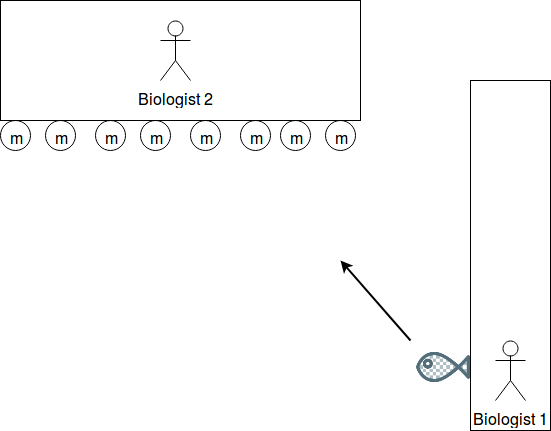
\includegraphics[width=\textwidth]{figures/porpoise_experiment1}
	\caption{Figure of testsetup of porpoise's echolocation. The two boxes indicate pierses, each with a biologist standing. On the piers 2, 8 hydrophones are mounted.}\label{usecase:porpoise_experiment1}
\end{figure}


Figure \ref{usecase:porpoise_experiment1} shows a porpoise swimming in a basin close to \textit{Biologist 1}.
When \textit{Biologist 2} throws bait in the basin, the porpoise will swim torwards the bait while emitting high frequency, narrow band clicks, in order to swim in the direction of the bait. A porpoise emits clicks at a frequency of $\approx$ 130 khz.
Since 8 microphones are mounted near the bait on piers 2, the recordingsystem is able to record the clicks emitted by the porpoise. This experiment exists in different variations where, for instance, different materials are mounted between the bait and the porpoise that tampers with the porpoise's clicks and hearing. The experiments are conducted using one batbox with 8 hydrophones.

These experiments use \textit{Trigger recordings} and \textit{Long recordings} as described in section \ref{sec:usecase:triggerrecording} and \ref{sec:usecase:longrecording} respectively.

\subsection{Live Underwater Laboratorium}
The biologists in Kerteminde has an ongoing project, where they want to enlighten students in folkeskoler and efterskoler about the nature under water. They want to to stream live sound from the ocean in Kerteminde. Furthermore, they want to show live measurements of salinity, Ph and temperature of the ocean to the students.
This system will also be used to investigate how ferries etc. affect the lives of the animals living in the ocean. Biologists usually do experiments of fish in captivity, but they know very little about the life in the ocean outside their window. Ideally the biologists wants to get an notification when a fish or animal of interest is located in the ocean around Fyn.


\subsection{Bats}
The biologists at SDU do experiments with bats to gain knowledge about how bats use their echolocation, where bats live, and where they live in the nature.
Some of the experiments are conducted as described in section \ref{sec:usecase:porpoise} with porpoises. Instead of doing the experiments in water, they are conducted in a batcage showed in figure \ref{fig:usecase:batcage}. When the bats fly towards the bait, the biologist can create a recording using the trigger mechanism, as described in \ref{sec:usecase:triggerrecording}.

\begin{figure}[!h]
    \centering
    \begin{subfigure}[b]{0.45\textwidth}
        \includegraphics[width=\textwidth]{figures/batcage_cross}
        \caption{Figure of batcage with existing system's microphone mount}
        \label{fig:gull}
    \end{subfigure}
    ~ %add desired spacing between images, e. g. ~, \quad, \qquad, \hfill etc. 
    %(or a blank line to force the subfigure onto a new line)
    \begin{subfigure}[b]{0.45\textwidth}
        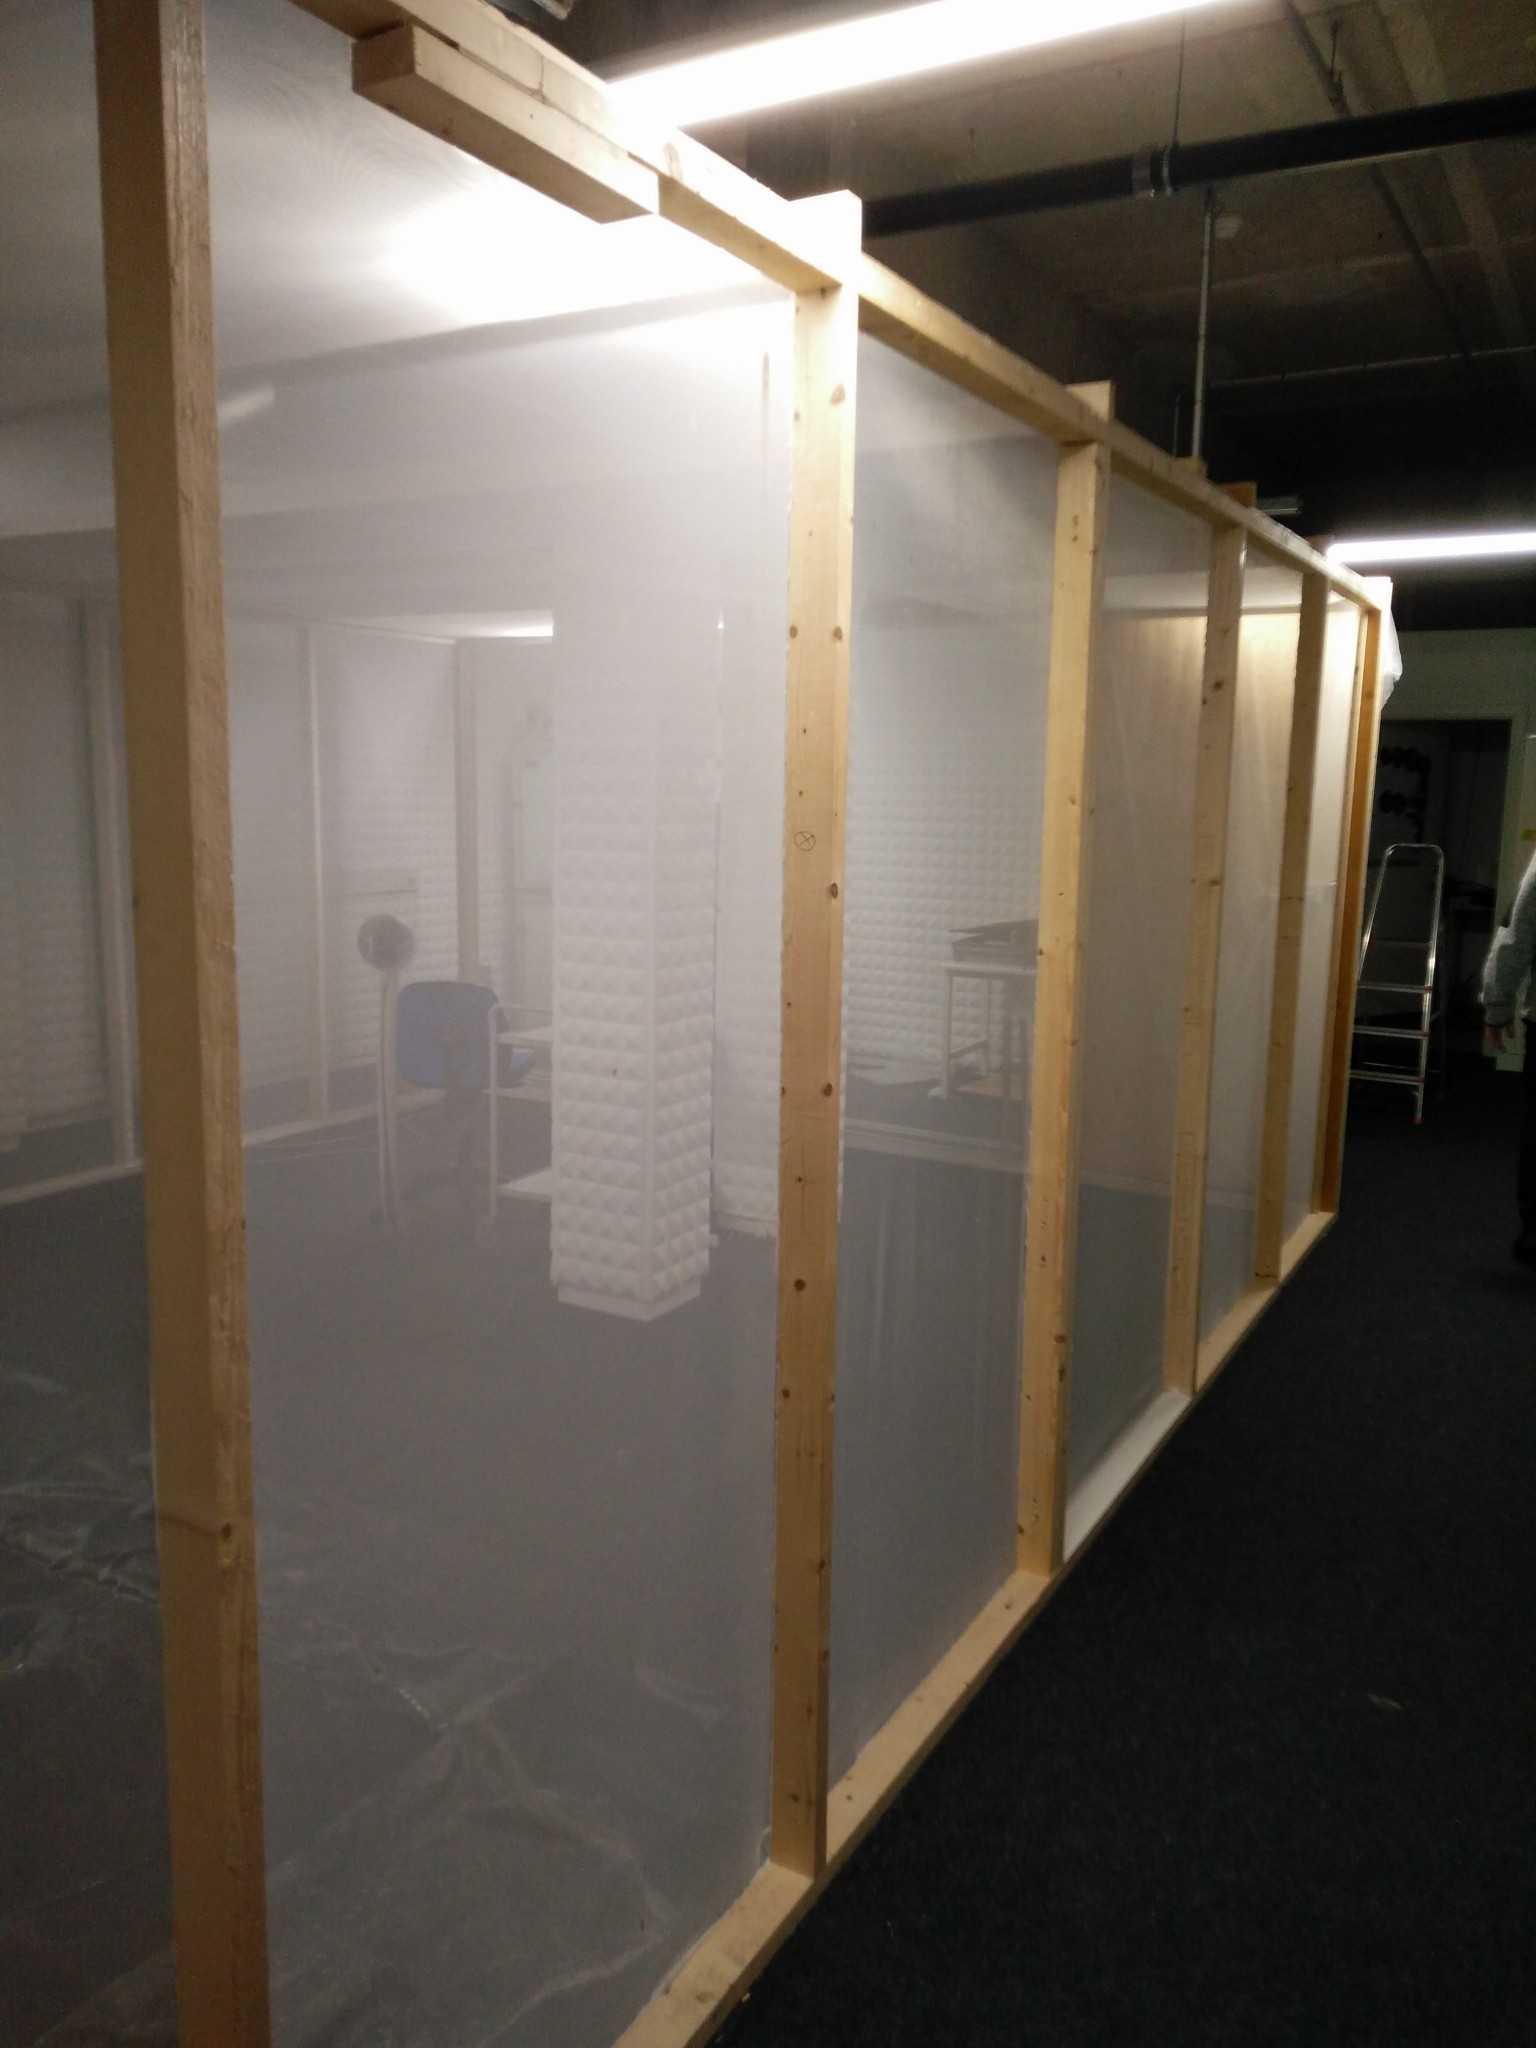
\includegraphics[width=\textwidth]{figures/batcage}
        \caption{Figure of the opposite end of the batcage}
        \label{fig:mouse}
    \end{subfigure}
    \caption{Pictures of batcage}\label{fig:usecase:batcage}
\end{figure}

Another set of experiments are conducted in panama. 8 microphones are mounted in a tree, in order to investigate which bat species live in the forest. As the microphones and the batbox is mounted in a forest, the batbox is running on battery. Due to the location of the recording system in a forest, it's cumbersome to get physical access to the system, to do maintenance like replacing battery, harddrives etc. The system do periodically \textit{short recordings} as described in section \ref{sec:usecase:shortrecordings}. 

A third experiment is done in Odense where the new hospital will be build.
%The idea is to investigate how the new hospital will affect the bats living in the area.
The idea is to put op N batboxes, each with 8 microphones in the area where the hospital will be build to get more knowledge about the bats that live in the area. During the conduct of the hospital and after the hospital has been build, the biologists want to know if the behaviour of bats have changed. The system should only do recordings in the nightly hour as bats are not active during daytime. This is described in section \ref{sec:usecase:shortrecordings}.

The biologists also have interest in mounting a batbox with a microphone on drones. An experiment is to manually steer a drone near a group of flying bats, to gain knowledge about how bats behave in the air, which species fly at different heights etc. This should in the future be automated such that two drones, each with 8 microphones and a batbox can point in the direction of the group of bats. In order to maintain the heading, the drones should emulate being a drone by emitting ultrasonic sounds which is then recorded by the microphones. The trigger recordings must be minimum 30 ms. To do this, processing of the recordings must be done online, as described in section \ref{sec:usecase:online}.
\todo{Question: App. where drones use echolocation?}
These experiments require long recordings as described in section \ref{sec:usecase:longrecording} in order to record while the drone is in the air and triggered-recording as described in section \ref{sec:usercase:longrecording} to listen for subsonic replies emitted by the drone.

\subsection{Frogs}
Biologists also have interest in recording frogs, in order to learn more about their vocalization capabilities. Frogs use advanced techniques to synchronize with other frogs, so they alternate vocalization to increase their change of being heard by females frogs. Furthermore they use techniques where they do vocalizing near a bigger male frog to amplify their vocalization to, as before, increase their change of getting hear by female frogs. Figure \ref{fig:usecase:frogs} shows an illustration of frogs vocalizing around a lake. Experiments are usually conducted by mounting 8 microphones and 1 batbox close to a lake. The system is running on battery and requires recording to be done in predefined period of time during daytime. This system requires short recordings as described in section \ref{sec:usecase:shortrecording}

\begin{figure}[H]
	\centering
	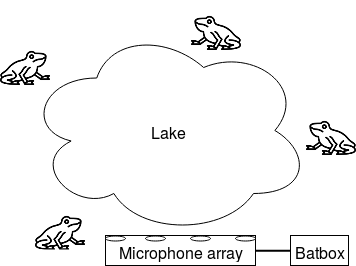
\includegraphics[width=0.6\textwidth]{figures/usecases_frogs}
	\caption{Figure of frogs sitting around a lake while the batbox is recording with 4 microphones} \label{fig:usecase:frogs}
\end{figure}

\subsubsection{Drones}
Drones are used to take pictures of the ocean, to see where porpoises are living. Drones will also be used in the future to investigate where salmon\todo{not salmon but?} breed in Denmark, as this is not known. Since the drone is hovering over the ocean, the biologists want to lower a hydrophone into the water from the drone, to listen to porpoises and other sea activity. This is sketched in figure \ref{fig:usecase:drone}.

\begin{figure}[h!]
	\centering
	
\includegraphics[width=0.4\textwidth]{figures/usecase_drone}
	\caption{Figure of the drone with a hydrophone hanging form the drone. The hydrophone is lowered into water to listen to sea animals}\label{fig:usecase:drone}
\end{figure}

In the beginning the system will only use one hydrophone, but in the future the might use more to do ecolocation to get the position of the sound source in the ocean.
The system will do short recordings as described in section \ref{sec:usecase:shortrecording}, as they only want to record if the drone detects any activity in the ocean.

\subsection{Zebra Finches}
Biologists use Zebra Finches for investigating vocalization, as the Zebra finch has a stereotypical sound. Especially the tutoring session between a young bird and its father has been investigated thoroughly. In an experiment, a teleconference system for birds has been build. The two birds are physically isolated in boxes,
but can communicate via cameras, screens, microphones and speakers. One batbox has been used, where 1 microphone is placed in each of the two boxes.\citep{larsen2016system}
Figure \ref{fig:usecases:zebra:overview} shows the conceptual design of the experiment:

\begin{figure}[h!]
	\centering
	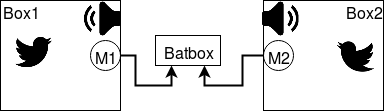
\includegraphics[width=0.6\textwidth]{figures/zebrafinches_experiment1.png}
	\caption{Pictures of experiment with zebra finches where only microphones, batbox and speakers are depicted}\label{fig:usecases:zebra:overview}
\end{figure}
It should be noted, that only two microphones are in use in this system.
As the system is designed to replay tutoring sessions from previous experiments, it is required that the system can replay recordings.
The system uses long recordings as described in section \ref{fig:usecase:longrecording}.


\begin{figure}
    \centering
    \begin{subfigure}[b]{0.3\textwidth}
        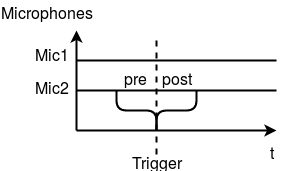
\includegraphics[width=\textwidth]{figures/recording_trigger.png}
        \caption{Trigger recording illustrated}
        \label{fig:usecase:triggerrecording}
    \end{subfigure}
    ~ %add desired spacing between images, e. g. ~, \quad, \qquad, \hfill etc. 
      %(or a blank line to force the subfigure onto a new line)
    \begin{subfigure}[b]{0.3\textwidth}
        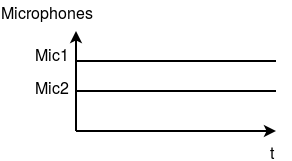
\includegraphics[width=\textwidth]{figures/recording_long.png}
        \caption{Long recording illustrated}
        \label{fig:usecase:longrecording}
    \end{subfigure}
    ~ %add desired spacing between images, e. g. ~, \quad, \qquad, \hfill etc. 
    %(or a blank line to force the subfigure onto a new line)
    \begin{subfigure}[b]{0.3\textwidth}
        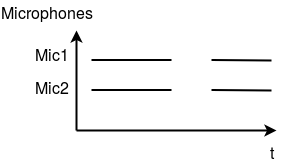
\includegraphics[width=\textwidth]{figures/recording_short.png}
        \caption{Short recording illustrated}
        \label{fig:usecase:shortrecording}
    \end{subfigure}
    \caption{Illustration of the three types of recordings}\label{fig:usecase:recordingtypes}
\end{figure}
\subsection{Long Recordings}\label{sec:usecase:longrecording}
Long recordings are used in experiments where it is required to do continuous recordings for, theoretically, indefinitely. Long recordings are used where either storage is always available or the local attached storage can be replaced when out of space. Long recordings  require external power is connected the system, and that it is not running on battery. A long recording is shown in figure \ref{sec:usecase:longrecording}.

\subsection{Trigger Recordings}\label{sec:usecase:triggerrecording}
Trigger recordings are used in experiments where it potentially takes a long time before the event of interest is happening. By using a trigger recording, the recording can be triggered after the event has happened, but where the event is saved in the recording. In figure \ref{fig:usecase:triggerrecording} two microphones are depicted with respect to time. When the system receives a trig, it will export the recording to the the biologist, starting at $trig-pre$ to $trig+post$. The duration of the recording will therefore be $pre+post$. The trig is usually received by a press on a button.

\subsection{Short Recordings}\label{sec:usecase:shortrecording}
Short recordings are used when the storage is limited or the batbox is not always powered up due to power constrains such as the batbox is running on battery. The start of the recording and duration must be specified such that the biologists can key in when the recordings should be conducted.
A short recording is depicted in figure \ref{fig:usecase:shortrecording}.

\subsection{Data Analysis}
%Analysis of recordings are usually done in one of three ways: online, offline or as batch processing.

By talking with biologists, the analysis of recording has been split into three groups: online, offline or batch processing.
\subsubsection{Online}\label{sec:usecase:online}
Online processing is when the processing is happening while the experiment is conducted. This implies that recordings and results can be used in the experiment such as in the \textit{Zebra Finches experiment}, where tampering with data online is important. Recordings can be saved, but is not required to. This also allows systems to only save the result of the processing meaning much less storage is needed.

\subsubsection{Offline}
Offline analysis is used in most use-cases where the recordings are saved to local storage. The processing of the recordings can be done when the storage is brought back from the test-location. When the recordings are replayed, it should emulate the online recordings.
It should be possible to replay the same recording multiple times, where it can be chosen when the replay should happen from. Furthermore it must be possible to specify the duration of the replay. It is required the replaying has a granularity of 1 second. In cases where multiple microphones or hydrophones together with sensors are recorded, it should be possible to specify which microphone or sensor to replay

\subsubsection{Batch Processing}
Batch processing is also happening offline, but in this case the recordings are exported as  files, which can be used on a supercomputer such as Abacus. The different between offline and Batch Processing is the fact, that in offline-analysis, the format of the recordings is raw and requires pre-processing.

\subsection{Overall Idea}
\subsection{Insert figures}



\section{MCLURS}

% The system supports sampling of 312.5 khz on each channel where the present version of the hardware has 8 channels. 
A recording system has been developed by John Hallam \& T{\'o}rur Andreassen \citep{andreassen2013ultrasonic} named Multi Channel Long-term Ultrasonic Recording System, which is used on most of the usescases list in section \ref{sec:usecase}. The hardware of MCLURS is described in section \ref{sec:currentsystem:hw}. 
However due to the MCLURS's design, it has some limitations which cannot be bypassed without redesigning the overall architecture. Limitations of the existing system is described in section \ref{sec:existingsystem:limitations}.\\


MCLURS is illustrated in figure \ref{fig:existingsystem:overview}. The yellow and blue boxes are hardware and software components respectively.
\todo{Fix figure colors. Yellow = hardware, blue = software}
\begin{figure}[h!]
	\centering
	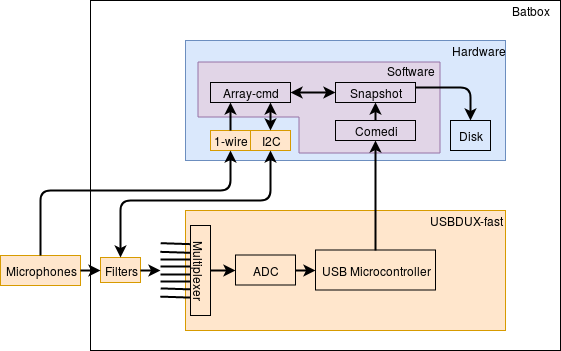
\includegraphics[width=1\textwidth]{figures/existing-system-overview.png} 
	\caption{Overview of existing system. Yellow boxes indicate hardware and blue boxes are software components.}\label{fig:existingsystem:overview}
\end{figure}
\todo{Ad line from USB Microcontroller to Multiplexer}

\todo{Add figure of three hardware components}

\subsection{Hardware}
The hardware used in MCLURS is shown in figure \ref{fig:existingsystem:hardware}.

\missingfigure{Hardware picture of (version 2B and droneboard)}

The hardware consists of 3 PCBs, each listed and described below:
\begin{enumerate}
	\item \textbf{Raspberry PI} The Raspberry PI runs the software described in section \ref{sec:existingsystem:software}. It interfaces the Miscellaneous PCB through GPIO headers on the RPI, and the USBDUX through USB.
	
	\item \textbf{USBdux-fast} The USBdux-fast board is responsible for sampling the 8 channels. The USBDUX-fast has an ADS807 ADC, which is a single channel ADC capable sampling at 53Mhz.\todo{Cite datasheet}.
Since the system has 8 channels, a multiplexer is placed in front of the ADC, that cycles through the 8 channel inputs.
The ADC and multiplexer is controlled by the onboard peripheral USB micocontroller(cy7c68013a) which instructs the ADC when to do sampling and the multiplexer to select channel. The microcontroller is running a firmware as explained in section\ref{sec:existingsystem:software:kernelmodule}.
	
	\item \textbf{Miscellaneous PCB} The Miscellaneous PCB is responsible for the 1W-interface to the microphones\todo{intorducte 1W somewhere}, the RTC, setting gain, filters, LEDs and proving power for the hardware
\end{enumerate}

Four versions of the hardware exists, however; changes from version 1 to version2B where bugfixes and addition of switch to control filters. The two relevant versions are \textit{Version 2B} and droneboard, as shown in figure \ref{fig:existingsystem:hardware:2B} and \ref{fig:existingsystem:hardware:droneboard} respectively.

\begin{itemize}
	\item \textbf{Version2B} Is the version used in existing usecases. 

	\item \textbf{Droneboard} Is to be used in usecase \ref{sec:usecase:drone}. This PCB is designed to be small and light, as it will be mounted on a drone as payload. The PCB is a merge of the \textit{Miscellaneous PCB} and USBDUX-fast, however the ADC has been replaced with a LC2205 that is 16 bits\todo{Cite datasheet}. Except for the size of a sample, the interface from the software perspective reminds the same as Version2B.

\end{itemize}
\myparagraph{Microphone}
Microphones connected to the MCLURS system usually have a small PCB build-in. The PCB contains a DS28E05\todo{Cite datasheet} 112-byte EEPROM, that allows setting microphone calibration parameters and microphone identifier. The microphone is showed in figure \ref{fig:existingsysem:hardware:microhpone}. The build-in PCB also contains circuitry that converts the single-ended output from the internal, actual mirophone into a differential output, in order to reduces the risk of electromagnetic noise.
\missingfigure{Figure of Microphone}

\subsubsection{Software Components} \label{sec:existingsystem:software}
MCLURS consists of a suite of programs, that all have a well defined responsibility. The programs are written in C where the program is time-critical or Perl, if the program is not time critical. \textit{array} is written in bash, as it is the CLI interface to MCLURS that allows starting recordings etc.

Below is listed the programs in MCLURS:
\begin{itemize}
	\item \textbf{snapchot} is responsible for getting the samples from the usbdux/comedi (see section \ref{sec:existingsystem:software:kernelmodule}) module and writing the samples into files. When snapshot is initialized, it will record samples, however data is only saved to a circular buffer until it is told to write the buffer into a file. The snapshot will save part of the circular buffer to a file when it receives a “snap” command. This gives the ability to get a recording, consisting of data from a predefined time before it receives the “snap” command. This makes up the \textit{trigger-recording}. Snapshot is designed to not miss out samples from the comedy device and there by not from the ADC. Snapshot supports long-recordings recordings, where it just repeats the triggering and saves each trig to a file.
	
	\item \textbf{grab} has overlapping responsibility with snapshot, however: grab outputs samples to stdout and not by writing to any files. Furthermore, the implementation of the grab node is much more simple, as it has no need to maintain a circular buffer and thereby implement less memory management. If the consuming process blocks its stdin, grab will loose samples. Grab is usually used to short/long-recordings.

	\item \textbf{snapchat} is responsible for communicating with snapchot and/or array-cmd depending on the usecase. Snapchat takes commands as input and forwards them to snapshot or array-cmd.

	\item \textbf{array-cmd} is responsible for:
	\begin{enumerate}	
		\item Setting up the USBDUX during startup of MCLURS 
		\item Handling GPIO to HMI
		\item Saving meta-data for recordings
		\item Determining mode of operation
		\item Handling connected microphones.
		\item Being the interface to the system using ZMQ and UDP.
		\item Hardware communication with DAC for filtering over I2C.
	\end{enumerate} \todo{Refer to appendix with flowchart of array-cmd}

	
	\item \textbf{trig} instructs the snapshot when to do a snapshot by constructing and sending a “snap” command to either cmd-array or snapchat. It can be told to do snaps repeatedly or only once a button has been pressed.

	\item {array} is a script that hides the complexity of the system to ease the interface for the biologists. It is capable of initializing the system, listing connected microphones, setting options on the microphones, starting/stopping recordings etc.

\end{itemize}


Table \ref{tab:existingsystem:software:nodes} lists the different programs and how they are run, in which language and when they are run. "Daemon" means the program is run under supervison from \textit{runit} and \textit{One-shot} means til program is run when needed.

\begin{table}[h!]
\centering
\resizebox{\textwidth}{!}{%
\begin{tabular}{|l|l|l|}
\hline
\textbf{Node name} & \textbf{Impl. Language} & \textbf{Running mode} \\ \hline
Snapshot           & C                       & Daemon                \\ \hline
Snapchat           & C                       & One-shot              \\ \hline
Grab               & C                       & One-shot              \\ \hline
Trig               & C                       & One-shot              \\ \hline
array-cmd          & Perl                    & Daemon                \\ \hline
array              & Bash                    & Oneshot               \\ \hline
\end{tabular}%
}
\caption{My caption}
\label{my-label}
\end{table}


%Hardware - trigger line(master/slave setups)

\myparagraph{Inter Process Communication}
The interface to the recording system is either UDP or ZMQ using request/reply-pattern. Communication between the demons and CLI tools is ZMQ. Communication between threads in snapshot is also using ZMQ, however using push-patterns as ZMQ is used to do logging from busy threads.

\myparagraph{Startup and Supervision}
All daemons are run under supervision from the debian runit package. The runit package is both responsible for starting the nodes during startup, but also to keep the nodes running in case one of them crashes. Since runit does not provide any control of the order of startup, some fiddling has been made in order to start the snapshot and array-cmd in the correct order. 


\todo{Describe and make diagrams of how to userlands tools talk through comedi modules to hardware}

\myparagraph{Kernel module} \label{sec:existingsystem:software:kernelmodule}
\begin{figure}[h!]
	\centering
	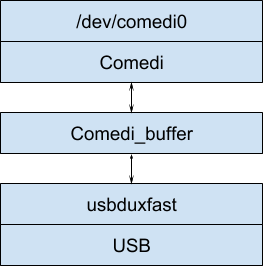
\includegraphics[width=0.5\textwidth]{figures/mclurs_comedi}
\end{figure}

\subsubsection{Limitations} \label{sec:exisingsystem:limitations}
An example of this is the need to show the operation on the system live. 
The software running on the system, is implemented on a single RPI. The RPI is designed such that the USB-ports and ethernet is connected to the USB-bus. When the ADC samples at it highest samplerate, it generates 5mb/sec which is.

\begin{itemize}
	\item Not capable of doing online processing of recordings.
\end{itemize}


\chapter{Analysis}
In order to develop and implement programs to send and receive streams, the requirements from the use cases must be extracted.
%Some requirements will be logical consequences or decisions in order to nail down details.
This section will constitute an analysis to such a degree where the design section can discuss which protocol(s) to use.

\section{Assumptions}
During the analysis, design and implementation sections the following assumptions have been made:
\begin{itemize}
	\item No packets are lost or corrupted during transmission.
	\item No bandwidth limitation exists on the network.
\end{itemize}

\todo{Discuss assumptions in \textit{Discussion}-section}
\section{Design Requirements}
The proposed system is designed with the concepts of the unix philosophy in mind
\begin{itemize}
	\item Programs should do one thing, and do it well
	\item Programs should be able to work together
	\item Programs should be capable of taking streams of text as input
\end{itemize}

By complying with the three ideas from above, the system should consist of multiple small programs that can be put together in different ways to serve different purposes.

Since the system is developed for biologists, it should be easy to use and require minimum intervention to get it running. Ideally the system should be “plug and play” such that biologists can take the number of recording boxes required for their application and put it all together without the need to configure software on any of the boxes. \todo{Add Extensibility somewhere, maybe not due to maintainability}

\todo{Stram op...}

\todo{Add: Write as little code as possible, use already existing code maintained by other developers}
\todo{add: Should be a requirement that it should be easy to write new nodes. Should not require an interface to send commands, should be self-contained as possible.}

Furthermore the system should also be:

\begin{itemize}
	\item Maintainability
As other people will improve the system in the future, it should also be easy to maintain. This will almost happen automatically if the “unix design rules” are kept in mind during design and development.
\item Modular
The system should consist of multiple small programs so that it can be used in all existing use-cases but also those that might come in the future.
\item Reusability
As much code should be as reusable as possible in order to avoid implementing the same functionality multiple times.
\item Extensible
    By implementing small programs, the system should be easy to extend in the future.
    If functionality is missing in one of the programs, it should be possible to create a new 
    program with the new functionality.
\end{itemize}

However splitting functionality into multiple modules will also be done with caution as it might come with the price of performance. Each time programs are split up, there is usually required some communication between the programs or some exchange of memory. The communication might turn out to be unnecessary performance consumption. Therefore splitting programs up is seen as simplicity(as it eases development and use) vs. performance.

% \section{Recording}
% stream data out
% timestamp for accurately compare streams\todo{verify with John}


\begin{figure}[h!]
	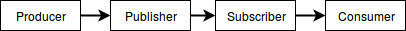
\includegraphics[width=1\textwidth]{figures/analysis-terminilogy-overview.png}
	\caption{Overview of nodes, to help the reader understand the terminology used throughout the following sections. It should be noted, that the producer and consumer is just programs producing and consuming streams without being aware of the protocols between the publisher and subscriber.}
\end{figure}

\section{Streams}
% A streams is an abstraction, that hides the details in the communication between subscribers and publishers.
A stream is defined as coherent data, which is in the process of being transmitted. A stream does not conceptually have an explicit beginning or end nor does it necessarily have a header explaining the content of the stream. A stream can either be continuous or discrete which depends on the content of the stream. 


Given use case \ref{usecase:x}, the stream must be capable of comprising sound, text and video formats only relying on codecs available. As all streams are transmitted over multicast groups, the streams must be packet-oriented since they are transported as UDP packets.
As UDP packets might arrive out of order, or not arrive at all, the stream must be robust to lost packets, without loosing global knowledge of the stream.
TCP is not considered an option, as this would not take advantage of the multicast groups. TCP is connection-oriented meaning it would require a connection from each producer to each consumer, this would limit the number of consumers per producer due to the RPI's bandwidth limitation.

All nodes that publish and subscrib is stateless with respect to the data streams. However, they might both maintain a state about the metadata streams.

Since the stream is just data, there must be metadata available that describes the content of the streams. The streams must be described unambiguously, such that each stream can be differentiated from the other streams. Since the streams are to be recorded and replayed, metadata must also be available when the streams are replayed, in order to identify the streams when replayed. Therefore, the streams must be complete and depend on no external knowledge.
As the system will usually comprise of multiple streams, each stream must have a unique, sensible name used to refer to the stream. Furthermore it must have an unique identifier that allow streams to refer to eachother.
As in use case \ref{usecase:energizer}, where a node consumes a stream and produces a new stream, the new stream must explicitly specify its parent stream using the parent's unique identifier. This gives rise to model the streams as a forest of graphs, where each graph should always be an directed acyclic graph, in order to avoid streams that depend on themselves.

\begin{figure}[h!]
	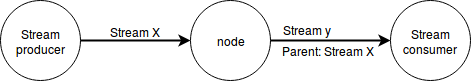
\includegraphics[width=1\textwidth]{figures/stream-graph}
\end{figure}

\section{Metadata}
\subsection{Introduction}\todo{Self-identifying streams in analysis}

By inspection of the use cases and the streaming analysis in section \ref{sec:analysis}, it has been decided to split metadata into tree categories:
\begin{enumerate}
	\item \textit{Essential metadata} which covers the metadata that is required to identify and decode the stream.
	\item \textit{Non-essential metadata} which is used between the producer and consumer. This metadata is only relevant to the users.
	\item \textit{Events} which describes an event in the stream. An event is defined as something interesting in the stream.
\end{enumerate}

\subsection{Event}
From use case \ref{usecase:batbox}, it is required that the system can handle events consisting of the following entries:
\begin{itemize}
	\item \textit{Start} States the absolute date and time of when the event appear. 
	\item \textit{Duration} States for how long time the event is active.
	\item \textit{Data} Associates data to the event. This can either be entered by a user or by a node on the network.
\end{itemize}

Given that streams are to be recorded replayable, the events must also be replayable while still relating to a stream and point in time explicit and unambiguously.

\subsection{Essential Metadata}
From the analysis of streams ~\ref{analysis:stream}, it is required that the streams are self-identifying to the subscriber. This implies that metadata that describes the properties of the stream must be available to the subscriber.
From analysis of streams ~\ref{analysis:stream:requirement:x}, it is required that subscribers can join a stream at any arbitrary time. In order for the subscriber to know the properties of the stream, the metadata must be retransmitted periodically. This metadata is essential in order to identify and decode the stream and will be referred to as "essential metadata".\\

\subsection{None-essential Metadata}
The existing batboxes provide metadata about the streams, which is not essential to identify or decode the stream but is relevant to the user or consumer. An example of this is listed below.
\begin{itemize}
	\item Batbox-uuid
	\item Batbox's filter settings
	\item Microphone parameters
\end{itemize} 
The publishers and subscribers must be agnostic to the semantics of this metadata, as it is provided by the producer and used by the consumer. The subscriber and publisher must allow for conversion between different formats used by the producer and consumer, in order to ease implementing producers and consumers.
%The subscriber and publisher must also be agnostic to the format of the metadata, as the producer and consumer might use XML, JSON, EMBL etc. to represent metadata.
This will be referred to as "none-essential metadata", as this metadata is not essential with respect to the streams.\\

\subsection{Metadata Format}
From the design requirements, the metadata must be extensible such that the structure and list of parameters can be adopted as needed.

Given the analysis and design requirements, it has been decided, that metadata is essentially hierarchical key-value structures, that can be represented in different formats. From that decision the following requirements are fulfilled:
\begin{itemize}
	\item Extensible - as new key-value pairs can be added as needed.
	\item Expressive - since associative arrays, arrays etc. can be expressed.
	\item Convertable - as both subscribers and publishers can convert into the format required by the consumer and publishers independently.
\end{itemize}

\section{Publishers \& Subscribers}
\subsection{Introduction}
The terminology used to describe streams throughout the analysis is used from RFC7656.

Nodes publishing streams will be referred to as publishers through the following sections. Nodes receiving streams will be referred to as a subscriber, as they subscribe to streams in order to get the streams. \\
A subscriber and publisher is depicted in figure \ref{fig:analysis:pubsub}.

\begin{figure}[h!]
    \centering
    \begin{subfigure}[b]{1\textwidth}
        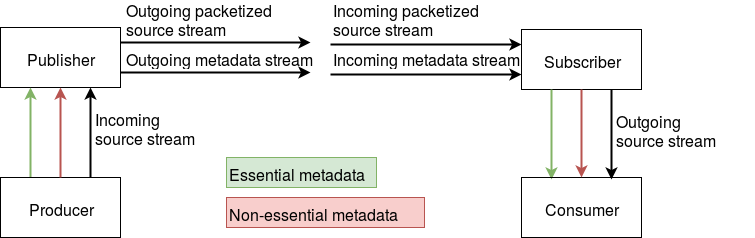
\includegraphics[width=\textwidth]{figures/publisher-subscriber}
    \end{subfigure}
     \caption{A publisher(left) and subscriber(right) depicted}\label{fig:analysis:pubsub}
\end{figure}

A source stream is defined as a stream of digital samples that has been synchronized with a reference clock and comes from a particular media source.

A packetized source stream is defined as a source stream where the stream is split into packets.
The outgoing source stream is identical to the oncoming source stream.
Non-essential metadata is as defined in \ref{sec:analysis:metadata}. Incoming none-essential metadata will be the same as the outgoing none-essential metadata.

The \textit{outgoing metadata stream} is \textit{none-essential} and \textit{essential metadata} combined as \textit{essential metdata} is used by the publisher and subscriber.

\subsection{Analysis}
As streams may contain different media, the publisher and subscriber must be agnostic to the codec of the stream, and must provide an interface to handle the data as well as metadata to and from the streams.
In order to allow multiple nodes to use a stream, multiple subscribers must be able to subscribe to the same multicast group. If a publisher publishes to a topic already in use, it must give a warning to the user. In order for this to work, the publishers and subscribers must implement a presence protocol, that detects the presents of other publishers and subscribers on a specific stream. This must be implemented in a way such that possible conflicts can be detected within X seconds from a publisher/subscriber is run, where X is specified as a parameter to the nodes.

As there is no designated master in the system, the publisher must be designed such that that independently can find available multicast groups, without relying on too many well-known multicast groups. When a subscriber is told to subscribe to a stream using the stream's unique name, the subscriber must single-handedly be able to find the requested multicast group.
As publishers and subscribers unlikely joins multicast groups at the same time, the publisher and subscriber most be able to cope with nodes asynchronously joining and leaving multicast groups.

Given design requirement X in section \ref{sec:analysis:designrequirements}, the publishers/subscribers must be opaque such that they encapsulate all of their internal protocols. In practice this means that the producers and consumers must be unaware of the communication between the subscribers and publishers.

%Both producer and consumer must be implemented as C-libraries and support bindings to other languages, to ease implementing new consumers and producers for future applications.

%The publishers and subscribers must react to

As metadata is required, it must be possible to provide metadata to the publishers such that it can stream it to the subscribers.
Given that the subscribers and publishers work on incoming data from either a stream or producer, they should only do work if 1) data from a stream is received or 2) the node must do work periodically.


\section{Historian}

Storing data is essential in all use cases, that require post-processing of recordings. Saving recordings to a local disk and later replay the recordings should be the only responsibilities of a designated node referred to as historian.
The historian should not be limited to record one stream, but should be capable of saving recordings from multiple streams. 

From use case \ref{sec:uc:x}, the historian should be able to save the following three types of recordings:
\begin{itemize}
	\item Long recordings
		In order for the node to save long recordings, it should be capable of writing to a local mounted storage periodically, and not store the entire recording in memory, as this would limit the maximum recording time.

	\item Short recordings
		With short recordings, the same applies as longtime recordings, however it should be possible to decide when and for how long time the recording should run. The historian must provide an interface that allows setting when to do recordings and for how long time.
	\item Trigger recordings
		From use case \ref{usecase:trig}, trigger recording is required. The historian must be able to replay a recording of arbitrary length at a arbitrary time of recorded data. This implies that the recording must support recording while replaying recordings. For this to work, it must be possible to specify which interface the historian should replay the recordings to.
\end{itemize}

As the node should be responsible for recording multiple streams, it should save the streams unambiguously with their associated metadata, such that the streams can be uniquely identified when replayed.
Given that streams can contain different media and encodings, the historian must be agnostic to the content of the stream.

Given that it might be possible that a stream must not be recorded, the historian must support ignoring streams that explicit states not to be recorded.



% Record multiple high and low bandwidth data streams


\subsection{Replaying}
Since the nodes processing the streams should be run when the streams are recorded, online or after the streams has been recorded, offline, the historian must replay the streams such that a processing nodes is unaware of the streams are live or replayed. This implies that the stream must be replayed in same order as it is recorded and in real-time meaning x seconds of recording takes x seconds to replay. Furthermore, this implies that metadata recorded must be replayed with the streams, also in real-time.
 From usecase \ref{sec:usecase:post-processing} it is required to be able to replay the same recordings multiple times. This implies that the historian must not delete the recordings after the recording has been played the first time.
As the historian saves streams and metadata with respect to time, the replaying must be started by requesting a replay from a given time and date. It should also be possible to send for how long the historian should replay, so that a replay will not default continue until stopped. For this to work, the historian must have an interface that allows requesting the following:


\begin{itemize}
	\item Date and time from where the historian should replay the streams.
	\item Selecting which streams to be replayed.
	\item To which interface the streams should be replayed. This will be useful in the use case \ref{usecase:trigger}, where requesting data might happen meanwhile the historian is recording.
	\item Replay rate that allows setting how fast the replaying should happen. 
\end{itemize}

As there is no guarantee that all batboxes are powered up when the historian starts recording, the historian must be able to autodiscover streams as they become available using the presence mechanism described in section \ref{sec:analysis:streams}.

The historian should not rely on specific hardware configuration. See section \ref{section:analysis:network} for analysis of required network.
 
\begin{enumerate}
	\item The historian must support recording multiple streams to local mounted storage.
	\item The historian must support replaying while recording.
	\item The historian must be agnostic with respect to the streams' encoding.
	\item The replayed streams must be unambiguous.
	\item The historian must replay streams with all of the streams' associated metadata.
	\item The historian must be robust to stream packets arriving out-of-order or never arriving.
	\item The historian must replay streams' packets in same order as they are recorded.
	\item The historian must ignore streams that explicitly states they should not be recorded.
	\item The historian must be able to replay streams and metadata in real-time, as they are recorded.
	\item The historian must not change the stream nor metadata during replaying.
	\item The historian must replay streams such that a processing-node cannot tell whether the stream is replayed or live.
	\item The historian must support replaying the same stream multiple times.
	\item The historian must have an interface that allows requesting:
	\begin{itemize}
		\item Date and time from where the historian should replay the streams.
		\item Selecting which streams to be replayed.
		\item To which interface the streams should be replayed. 
		\item Replay rate that allows setting how fast the replaying should happen. 
		\item How many packet should be replayed.
		\item When the historian should record and for how long time.
	\end{itemize}
	The historian must not rely on specific hardware with specific properties.
	The historian must be able to discover streams as the streams appear on the network.
\end{enumerate}

Given the limited time, the requirements has been prioritized into \textit{Need to have} and \textit{Nice to have} in table \ref{sec:analysis:historian:tablefeatures}.
\begin{table}[h!]
\centering
\caption{Table prioritizing the requriements into nice-to-have and must-have}
\label{sec:analysis:historian:tablefeatures}
\begin{tabular}{l|l|l}

\multicolumn{3}{l}{Need to have}              \\ \hline
----------  & --------- & ---------------------------------- \\ \hline
----------- & --------  & --------------------------------- \\ \hline
\multicolumn{3}{l}{Nice to have}              \\ \hline
            &           &                       \\ \hline
            &           &                       \\ \hline
\end{tabular}
\end{table}

\section{Energy Calculator}
\textbf{Just some notes}
% Node responsible for calculating energy in signal. 
From use case \ref{sec:usecase:energizer}, the energy calculation should happen from bulk of samples corresponding to 1 ms. To ease the implementation of the energizer-node and future nodes, it should be possible to set the payload size of the publisher node. If the payload length of the stream corresponds to 1 ms of samples, the energizer node do not have to implement a buffer mechanism. If the length of the packet exceeds the practical limits of the network, the producer must give a warning. From the incoming data to the producer, and the outgoing data from the consumer, there should be no limit of the packet sizes.

\section{Network}
As all streams leaving the nodes are timestamped, there is no restrictions on how the devices should be connected on the network. Packets can go through different number of hobs without causing problems, if the timestamps from the streams are used, and not the order the packets are leaving the historian during replay.

To connect multiple hosts on the network, multiple switches can be connected together. If multiple switches are connected, the bandwidth between switched should be handled with care. Each batbox generates 40 Mbit/s of data, so if a 24 ports switch is used to connect 23 batboxes and one historian, the link between the switch and the historian must be 1 Gbit. If an 48 ports switch is used, 1.8 Gbits is required between the switch and the historian. It should be noted, that a switch's non-blocking capacity, meaning the bandwidth it can handle at the same time, rarely equals the (number of ports) x (the bandwidth of each port).

Each switch must support the following features in order to handle IPv6 multicast traffic properly.

\begin{itemize}
	 \item IGMP snooping, in order to avoid broadcasting multicast traffic.
	 \item MLD, protocol used by IPv6 to join and leave multicast groups.
\end{itemize}

If the system scales out enough, limitations might arise, however these are not seen as realistic limitations.

\todo{must support running on virtual interfaces}

\subsection{Requirements}
From the analysis, the following requirements can be extracted.
\subsubsection{Streams}
\begin{enumerate}
	\item The stream can be either continuous or discrete.
	\item The stream must comprise different datatypes only by relying on available codecs.
	\item The stream must be packet-oriented and stateless
	\item The stream must be transported over UDP
	\item The stream must be robust to UDP packets that arrive out of order or never arrive.
	\item The stream must be represented unambiguously
	\item Metadata must be provided by the publishers and be available to the subscribers 
\end{enumerate}
\todo{Table of requirements[Where it's defined][Where it's tested][Whether it passes}

\subsubsection{Producer \& Consumer}
\begin{enumerate}
	\item The producer and consumer must be agnostic to the stream's payload.
	\item Multiple producers must send to the same multicast group.
	\item Multiple consumers must receive from the same multicast group.
	\item The producers and consumers must implement a presence mechanism to know about other producers and consumers.
	\begin{enumerate}
		\item It must takes a finite maximum number of seconds for a producer or subscriber to know who is present. The max time must be a parameter of each node.
		\item It must take a finite maximum number of seconds for a producer or consumer to detect whether a multicast group is in use, and if yes, by whom.
		\item It must assume nodes leaving a multicast group sends a "bye".
		\item It must be robust to "bye"-messages not arriving to all nodes.
		\item It must handle nodes joining and leaving at any arbitrary time.
	\end{enumerate}
	\item The producers must be able to find unused multicast groups single-handedly.
	\item Given a unique name of a stream, the consumer must be able to resolve the multicast address of the stream.
	\item Both producers and consumers must be able to cope with nodes joining asynchronously.
	\item The producer and consumer must be implemented in C and support language bindings.
	\item The payload length of the stream should be adjustable as a parameter on the producer nodes.
		\begin{enumerate}
			\item If the requested payload size is exceeded practical limits, a warning must be given.
		\end{enumerate}
	\item There should not be a limit of the packet size of the incoming data to the producer, or outgoing data from the consumer.
	\item The producer must support streaming provided metadata to the consumers.
	\item Both producer and consumer must be agnostic with respect to the semantics of the metadata.
\end{enumerate}

\subsubsection{Metdata}

\begin{enumerate}
	\item Metadata must unambiguously relate to the continuous data stream.
	\item Metadata must be expressive.
	\item Metadata must be convertable.
	\item Metadata must be extensible.
	\item Metadata must be complete.
	\item Metadata must be hierarchical key-value pairs.
	\item The publisher and subscriber must be capable of converting between metadata formats.
	\item Events must have a start time and date
	\item Events must have a duration.
	\item Events must contain data relating to the event.
	\item Essential metadata must be retransmitted periodically
	\item None-essential metadata must be retransmitted periodically
\end{enumerate}

\subsubsection{Historian}

\chapter{Design}

% http://www.faqs.org/rfcs/rfc5219.html <- mp3 i rtp
% RTP description https://flylib.com/books/en/4.245.1.27/1/
Video conference system(VCS) utilize audio and video streams, as a video conference is a connection between people residing in separate locations. This connection gives the impression that people participating in the video conference are present in the physical meeting. VCS usually allows for multiple participants to join a meeting where all participants are able to see each other. CVS might allow control of the camera by the remote participant in order to look at the person who is currently speaking. 
Lip-sync is often preferred during the video conference, to further give the impression the remote-participant is present. Lip-sync is when the sound from the remote participants is synchronized with the video stream. This usually has to be implemented by the streaming protocols as sound and video is not necessarily transmitted in the same stream and there by not synchronized when received by the recipient.

\missingfigure{sketch of video conference}

VCS usually utilizes the protocols shown in table ~\ref{table:vcs:protocols}. Proprietary VCSs such as Skype use closed protocol specifications which is not included in the table.


\begin{table}[]
	\centering
	\resizebox{\textwidth}{!}{%
		\begin{tabular}{@{}|l|l|l|l|@{}}
			\toprule
			\textbf{Protocol}             & \textbf{Abreviation} & \textbf{Described in} & \textbf{Note} \\ \midrule
			Realtime Transport Protocol   & RTP                  &                       & Transports video, sound etc.\\ \midrule
			RTP Control Protocol          & RTCP                 &                       & Quality feedback, participant identification and timing\\ \midrule
			Session Description Protocol  & SDP                  &                       & Describes a RTP session\\ \midrule
			Session Announcement Protocol & SAP                  &                       & Announces a SDP on multicast group\\ \bottomrule
		\end{tabular}%
	}
	\caption{Table showing protocols usually used in a video conference system.}
	\label{my-label}
\end{table}
\todo{Add RTSP and other non-relevant protocols?}

\section{Real-time Transport Protocol}
The RTP protocol is a network protocol for transmitting audio and video data in Voice-over-IP(VoIP), video conferences and online services that require streaming media. RTP is usually run over UDP, however it might be used over TCP as well.
A RTP session consists of one or more participants who are communicating using RTP. A participant may be active in multiple RTP sessions e.g. one session for streaming audio data and another session for streaming video data. For each participant, the session is identified by an IP and port pair to which data should be sent, and a port pair on which data is received. 

The RTP packet is depicted below:

\begin{figure}[h!]
\begin{verbatim}
    0                   1                   2                   3
    0 1 2 3 4 5 6 7 8 9 0 1 2 3 4 5 6 7 8 9 0 1 2 3 4 5 6 7 8 9 0 1
   +-+-+-+-+-+-+-+-+-+-+-+-+-+-+-+-+-+-+-+-+-+-+-+-+-+-+-+-+-+-+-+-+
   |V=2|P|X|  CC   |M|     PT      |       sequence number         |
   +-+-+-+-+-+-+-+-+-+-+-+-+-+-+-+-+-+-+-+-+-+-+-+-+-+-+-+-+-+-+-+-+
   |                           timestamp                           |
   +-+-+-+-+-+-+-+-+-+-+-+-+-+-+-+-+-+-+-+-+-+-+-+-+-+-+-+-+-+-+-+-+
   |           synchronization source (SSRC) identifier            |
   +=+=+=+=+=+=+=+=+=+=+=+=+=+=+=+=+=+=+=+=+=+=+=+=+=+=+=+=+=+=+=+=+
   |            contributing source (CSRC) identifiers             |
   |                             ....                              |
   +-+-+-+-+-+-+-+-+-+-+-+-+-+-+-+-+-+-+-+-+-+-+-+-+-+-+-+-+-+-+-+-+
\end{verbatim}
\caption{Box in an old RFC}
\label{fig:ascii-box}
\end{figure}

many applications
profile
 - static
data types
Timestamp is a 32 bit value.
Id
source
yada..

\subsection{RTP payload}

It is important to be aware of the limits of the RTP protocol specification because it is deliberately incomplete in two ways. First, the standard does not specify algorithms for media playout and timing regeneration, synchronization between media streams, error concealment and correction, or congestion control. These are properly the province of the application designer, and because different applications have different needs, it would be foolish for the standard to mandate a single behavior.
The RTP protocol does not specify how the data should be packet into the payload of an RTP packet. This is defined by profiles and packet types. A profile can contain multiple data formats, and might describe some general details about the content of the RTP packet.
The most used profile is the "RTP/AV audio video for conference with minumal control", which is used for streaming audio and video.
RTP contains packet-type field.

\cite{perkins2003rtp}
\section{Real-time Control Protocol}
RTCP is used to provide reception quality feedback, participant identification, and synchronization between media streams. RTCP runs alongside RTP and provides periodic reporting of this information. Although data packets are typically sent every few milliseconds , the control protocol operates on the scale of seconds. The information sent in RTCP is necessary for synchronization between media streams ”for example, for lip synchronization between audio and video ”and can be useful for adapting the transmission according to reception quality feedback, and for identifying the participants . 

receiver report (RR), sender report (SR), source description (SDES), membership management (BYE), and application-defined (APP). 

\section{Session Description Protocol}
\todo{Description of SDP}

\subsection{Session Announcement Protocol}
\todo{Description of SAP}


\section{Gstreamer}
\todo{Describe gstreamer + pros and cons}


\section{Custom Implementation}
Implement using oRTP to do language binding to e.g. perl (Net::RTP)
\chapter{Implementation} \label{chp:implementation}
This chapter will describe the implementation of the \pub{} and \sub{} as designed in the chapter \ref{chp:design}.\todo{Maybe add some more}. When referring to a requirement from the design chapter, the reference will be e.g. P1 and S1 for the \pub{} and \sub{}, respectively.

\section{Software Components}
The \pub{} and \sub{} has been implemented in PERL, as PERL is a nice language to make proof-of-concept implementations. PERL uses CPAN \footnote{\url{https://www.cpan.org/}} as package library meaning many modules are available for timeconversion, protocols etc. PERL is chosen as it is the preferred scripting language by the author and because its an exiting language to truly master.\\

\noindent{}\pro{} and \cons{} written for testing is implemented in BASH, however as described, any scripting as well as programming language could be used.\\

\noindent{} The \pro{} used for interacting with \program{Snapshot} is written in PERL as existing PERL code were available for talking to the \program{Snapshot} daemon.

\subsection{RTP/RTCP}
In order for the \pub{} and \sub{} to support sending and receiving RTP and RTCP messages a library should be used, in order not to implement parsing and composing of messages. By research, two C libraries have been found and compared. As PERL has support for wrapping C/C++ into PERL modules, one of the two modules can be integrated into the \subs{} and \pubs{}. The two libraries are oRTP and jrtplib.\\

\noindent{}\myparagraph{oRTP} 
The oRTP library is used in \textit{linphone Open-source VoIP}, which is an open-source VoIP solution created and maintained by Belledonne Communications. The oRTP library is released under the GNU GPLv2 and proprietary license meaning the library can be used for open-source projects and in proprietary solutions.
The oRTP library implements RFC3550 with an API that offers a high as well as low level interfacing for sending and receiving RTP and RTCP packets and parsing and composing RTP and RTCP packets. It supports multiple RTP sessions with IPv4 and IPv6 unicast and multicast. Furthermore, it offers support for different profiles, meaning a custom profile can be implrunmodeemented.  oRTP has a sparse documentation with only an autogenerated doxygen, where most of the functionality is described. The source-code comes with simple examples, that explains some of the library's functionality. The library is written in C and can be found in Ubuntu and Debian's packet repository. At the time of writing, the latest commit on their official github has been made 24 days ago which indicates the project is active. In CPAN, an oRTP library can be found, that implements some of the most high level API functions.


\myparagraph{jrtplib}
The jrtplib library is developed at the the Expertise Centre for Digital Media (EDM), a research institute of the Hasselt University. At the time of writing the library has been used in 61 projects listed on \href{http://research.edm.uhasselt.be/jori/cgi-bin/listprojects.py?name=jrtplib}{Project list}. The library is free to use, but must include disclaimer in the source code. The library implements RFC3550 and provides primarily a high level API, that hides most of the implementation details. The library supports parsing, composing, sending and receiving RTP and RTCP messages but does not not implement any profile, The library is written in C++ and well-documented by giving a thoroughly \textit{Getting Started} and includes 7 examples showing how to utilize the functionality of the library. Unfortunately, at the moment of writing the maintainers have not done any commits for the past year.

The libraries are compared based on the following requirements:
\begin{itemize}
	\item \textit{In repository}: From design requirement 4, the library should, if possible, be in the Debian repository.
	\item \textit{RTCP impl.}: The library should implement RTCP, as RTCP is required by the \pub{} and \sub{}.
	\item \textit{Low level API}: As the \pub{} and \sub{} should send RTCP SDEs, RTCP, BYE and RTCP SR.
	\item \textit{Custom RTP Profile}: The library should allow using a custom profile, as the \pub{} and \sub{} requires a custom profile for the non-essential/essential metadata.\todo{Verify requirement}
	\item \textit{API documented}: Preferable to ease implementation of the \pub{} and \sub{}
	\item \textit{Actively Maintained}: Relatively important, in case bugs are discovered.
	\item \textit{IPv6/4 multicast support}: Required by requirement X \todo{Analysis requirement}
	\item \textit{Existing per-binding}: As the \pub{} and \sub{} will be implemented in perl, existing bindings are preferable to ease implementation.
	\item \textit{Multiple RTP session}: Required by design requirement X
	\item \textit{Send \& Receive RTP/RTCP}: is required by \pub{} and \sub{}, respectively.
	\item \textit{Includes examples}: Preferable as it eases implementation.
\end{itemize}

\begin{table}[H]
\centering
\begin{tabular}{@{}|l|l|l@{}|}
\hline
\multicolumn{1}{|l|}{\textbf{Library property}} & \multicolumn{1}{|l|}{\textbf{oRTP}}         & \multicolumn{1}{|l|}{\textbf{jrtplib}}       \\ \midrule
\multicolumn{1}{|l|}{In repository}    & \multicolumn{1}{c|}{\checkmark} & \multicolumn{1}{l|}{} \\ \midrule
\multicolumn{1}{|l|}{RTCP impl.} & \multicolumn{1}{c|}{\checkmark} & \multicolumn{1}{c|}{\checkmark} \\ \midrule
\multicolumn{1}{|l|}{Low level API} & \multicolumn{1}{c|}{\checkmark} & \multicolumn{1}{c|}{} \\ \midrule
\multicolumn{1}{|l|}{Custom RTP Profile} & \multicolumn{1}{c|}{\checkmark} & \multicolumn{1}{c|}{} \\ \midrule
\multicolumn{1}{|l|}{API documented}          & \multicolumn{1}{c|}{\checkmark} & \multicolumn{1}{c|}{\checkmark} \\ \midrule
\multicolumn{1}{|l|}{Actively Maintained}           & \multicolumn{1}{c|}{\checkmark} & \multicolumn{1}{l|}{} \\ \midrule
\multicolumn{1}{|l|}{IPv6 multicast support}           & \multicolumn{1}{c|}{\checkmark} & \multicolumn{1}{c|}{\checkmark} \\ \midrule
\multicolumn{1}{|l|}{IPv4 multicast support}           & \multicolumn{1}{c|}{\checkmark} & \multicolumn{1}{c|}{\checkmark} \\ \midrule
\multicolumn{1}{|l|}{Existing perl-binding}           & \multicolumn{1}{c|}{\checkmark} & \multicolumn{1}{c|}{} \\ \midrule
\multicolumn{1}{|l|}{Multiple RTP sessions support}           & \multicolumn{1}{c|}{\checkmark} & \multicolumn{1}{c|}{\checkmark} \\ \midrule
\multicolumn{1}{|l|}{Send \& Receive}           & \multicolumn{1}{c|}{\checkmark} & \multicolumn{1}{c|}{\checkmark} \\ \midrule
\multicolumn{1}{|l|}{Includes examples}           & \multicolumn{1}{c|}{\checkmark} & \multicolumn{1}{c|}{\checkmark}  \\ \bottomrule
\end{tabular}
\caption{Comparesion of oRTP and jrtplib}
\label{sec:implementation:rtplib}
\end{table}

Based on the number of checkmarks in table \ref{sec:implementation:rtplib}, it has been chosen to use the oRTP library.

\todo{File tree, describe common perl library}
\subsection{Publisher \& Subscriber}

\textit{P1: The \pub{} should be the logical master of the \pro{}}\\
\textit{S1: The \sub{} should be the logical master of the \pro{}}\\

From requirement P1,S2 the \pub{} and \sub{} being the logical masters has been implemented by passing the path to the \con{} and \pro{} to the \sub{} and \pro{} respectively as an argument. This design allows the \pub{} and \sub{} to pass the pipes to the \pro{} and \con{} during run of the \con{} and \pro{}, respectively.

\begin{listing}[H] 
\begin{minted}{python}
./publisher.pl --producer producer.pl -- -v
./subscriber.pl --producer consumer.pl -- -v
\end{minted}
\caption{Example of publisher.pl run with producer.pl as parameter}
\label{code:critical_section_c}
\end{listing}

This will result in the process tree as depicted in figure \ref{sec:implementation:runmode}.

\begin{listing}[H] 
\begin{minted}{python}
/usr/bin/perl publisher.pl --producer producer.pl
 \_ /usr/bin/perl producer.pl /tmp/pub_data_pipe /tmp/pub_metadata_pipe -v
 
 /usr/bin/perl subscriber.pl --consumer consumer.pl
 \_ /usr/bin/perl consumer.pl /tmp/pub_data_pipe /tmp/pub_metadata_pipe -v
\end{minted}
\caption{Example of publisher.pl run as logical master of the producer.pl}
\label{sec:implementation:runmode}
\end{listing}

By running the consumer and producers this way gives modularity in the way the programs can be run, and does not restrict how the \con{} and \pro{} should be implemented.
Three examples shows how the \pros{}, \cons{}, \pros{} and \subs{} can be integrated with MCLURS and the streaming idea in section \ref{sec:streamingidea}.

\myparagraph{Grab with Static Metadatafile}
If \program{Grab} is used to produce data, the \con{} can be written as shown in listing \ref{lst:implementation:grab}. It should be noted that the \pro{} is a thin layer around \program{Grab}, that simply attaches \program{grab}'s stdout, to the data pipe. See section \ref{sec:implementation:ipc} for more information about the named pipes.

\begin{listing}[H] 
\begin{minted}{bash}
#!/bin/bash
# Named pipes passed as parameters
DATA_PIPE=$1
MD_PIPE=$2

# Provide feedback to the user
echo "Starting producer"

# Set non-essential metadata to Publisher
cat metadata_example.json > $MD_PIPE

# Capture samples and write to datapipe with Fs of 250kHz
/usr/bin/grab -f 2500000 > $DATA_PIPE
\end{minted}
\caption{The listing shows an implementation of a \pro{} that writes metadata and samples to the datapipe and metadatapipe, respectively}
\label{lst:implementation:grab}
\end{listing}

\noindent{}Listing \ref{lst:implementation:grab} shows how the \pro{} could be integrated with \program{grab}.
Metadata is provided by reading the \textit{metadata\_example.json}, and writing it to the metadatapipe.
As \program{grab} does not provide timing of the samples, no RTCP SR messages can be sent.


\myparagraph{Snapshot with Dynamic Metadata}
In order to use the \pub{} and \con{} with \program{Snapshot}, the \pro{} must instruct \program{Snapshot} to do repeating snapshots. Furthermore, the \program{Snapshot} must be told where it should write the samples to. This is shown as pseudocode in listing \ref{lst:implementation:snapshot1}.

\begin{listing}[H] 
\begin{minted}{python}
# Named pipes passed as parameters
DATA_PIPE=$1
MD_PIPE=$2

open MD_PIPE
write metadata.json to MD_PIPE

snapshot = ZMQ(SNAPSHOT)
snapshot.setup()
snapshot.start()
snapshot.snap(start=0,length=4096,count=100,stream=\$1)

PeriodicRun(1, updateNonessentialMetadata());


def getNonessentialMetadata():
	metadata = snapshot.getNonessentialMetaData()
	write metadata to MD_PIPE
	
\end{minted}
\caption{The listing shows an implementation of a \pro{} that writes metadata and samples to the datapipe and metadatapipe, respectively}
\label{lst:implementation:snapshot1}
\end{listing}

The setup(), start() and snap() methods implement commands used by \program{Snapshot}, in order to set parameters, start recordings and write snapshots to the pipe.
A periodic timer is created at line 16, which periodically queries the \program{Snapshot} daemon, in order to get timing information. From design requirement P10, the RTCP SR packets should be sent in order to timestamp the data stream. In order to do this, \program{Snapshot} supports ZMQ clients to query for timing information. When a \textit{Ztatus} command\footnote{Command implemented by the \program{Snapshot} daemon} is received, it sends a reply of the following format:


\begin{listing}[H] 
\begin{minted}{python}
OK Ztatus: WRITER Files 0, Xfr space 49152[ki spl]
READER ACTIVE hix: 0x0000000000824800 [spl]\ 
  tix: 000000000000000000 [spl] now: 0x00002c8008e4ee1e [ns]
\end{minted}
\caption{The listing shows an implementation of a \pro{} that writes metadata and samples to the metadatapipe and datapipe, respectively}
\label{lst:implementation:snapshot1}
\end{listing}

The important part of the reply is the \ac{HIX} and ''now``. ''Now`` is a monotonic timestamp starting at a random value, which corresponds to the \ac{HIX}. Conversion of this information into RTCP SR packets is described in section \ref{sec:design:rtcpsr}.

The converted timestamp and associated \ac{HIX} is sent via the metadatapipe as shown in line 18 to the \pro{}. In this case, the \pro{} is more than a thin layer, but it should be noted that the \pro{} never handles the data, it only parses the pipe to the \program{Snapshot}.
Figure \ref{fig:implementation:dynamicmetadata} shows how the \pub{} interacts with the \pro{} which again interacts with the \program{Snapshot} daemon.


\begin{figure}[H]
    \centering
    \begin{subfigure}[b]{0.45\textwidth}
        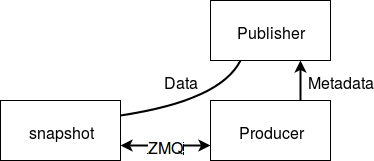
\includegraphics[width=\textwidth]{figures/impl_example_snapshot_overview}
        \caption{The figure shows the communication channels between the \pub{}, \pro{} and \program{Snapshot} daemon.}
        \label{fig:implementation:dynamicmetadata}
    \end{subfigure}
    ~ %add desired spacing between images, e. g. ~, \quad, \qquad, \hfill etc. 
      %(or a blank line to force the subfigure onto a new line)
    \begin{subfigure}[b]{0.45\textwidth}
        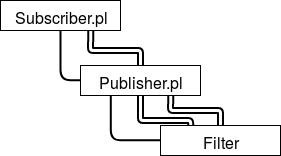
\includegraphics[width=\textwidth]{figures/impl_example_filter_overview}
        \caption{The figure shows the \textit{filter} is run by the \pub{} which is run by the \sub{}}
        \label{fig:implementation:filer}
    \end{subfigure}
\end{figure}

\myparagraph{Subscriber and Publisher with Filter}
As shown in the streaming idea section \ref{sec:streamingidea}, the system should be capable of handling a node that subscribers to a stream, and produces a new one. This will now be referred to as a filter. This can be done as showed in figure \ref{fig:implementation:filer}. In order to do do this, the \sub{} should take the \pub{} as argument, which takes the filter as argument. Unfortunately this does not work just by running the programs as described, a thin  later encapsulating the \pub{} has to be used. Listing \ref{lst:implementation:filterrun} shows how the three commands should be invoked.


\begin{listing}[H] 
\begin{minted}{bash}
perl subscriber.pl --consumer publisher.sh -- --producer filter
\end{minted}
\caption{The listing shows how a filter can be run, using the \textit{publisher.pl} and \textit{subscriber.pl}}
\label{lst:implementation:filter}
\end{listing}

If the above command is run, the process tree in listing \ref{lst:implementation:filtertree} should be seen. Due to lack of time, this has not been tested.

\begin{listing}[H] 
\begin{minted}{bash}
/usr/bin/perl subscriber.pl --consumer publisher.sh -- --producer filter
\_/bin/bash publisher.sh /tmp/datapipe1 /tmp/mdpipe1 --producer filter
  \_ /usr/bin/perl publisher.pl --producer filter -- /tmp/datapipe1 /tmp/mdpipe1
    \_./filter /tmp/datapipe2 /tmp/mdpipe2 /tmp/datapipe1 /tmp/mdpipe1
\end{minted}
\caption{The listing shows how a filter can be run, that reads data and metadata from two pipes, and writes new data and metadata to two new pipes}
\label{lst:implementation:filter}
\end{listing}
As mentioned, a bash script must be implemented, that takes the first two arguments, the datapipe and metadatapipe, and passes them to the \textit{Publisher.pl} after the $--$. If this layer is not used, the two pipes will be passed to the \textit{Publisher.pl} and not the \textit{Filter}, At the end, \textit{filter} receives four pipes, two for data and metadata input and two for data and metadata output.

\subsection{RTCP SR Timing} \label{sec:design:rtcpsr}
In order to calculate the 64 bit NTP timestamp for the RTCP SR packet, some calculations and time conversions must be done. As mentioned in the previous, the \program{Snapshot} reports a time and \ac{HIX}. This is depicted in figure \ref{fig:implementation:rtcpsr}.\footnote{This figure is a redrawing of a sketch made by John Hallam}
\begin{figure}[H]
	\centering
	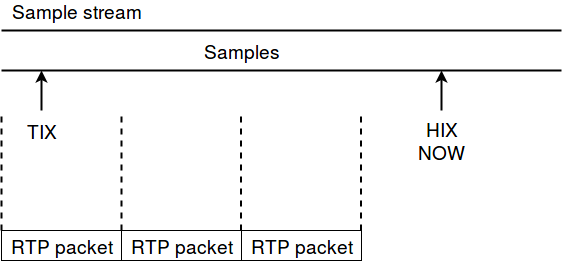
\includegraphics[width=0.9\textwidth]{figures/rtcp_sr_timing}
	\caption{The figure shows the samples in a stream, with head(HIX) and tail(TAI) pointers. It should be noted that the ''now`` is when sample pointed to by HIX is captured}\label{fig:implementation:rtcpsr}
\end{figure}

\program{Snapchat} timestamps the sample using CLOCK\_MONOTONIC meaning the clock has a random offset but is always increasing and is thereby not affected by \ac{NTP} updates. In order to use the timestamp, this random offset has to be calculated. This calculation is shown below.

\begin{align}
	mon_1 &= parse(Ztatus).now \\
	realtime &= \text{now in UTC in seconds since epoch} \\
	mon_2 &= parse(Ztatus).now \\
	\text{UTC\_offset} &= realtime-(mon_1+mon_2)/2 
\end{align}
By getting the monotonic time before and after taking the realtime clock in UTC, the offset can be estimated by calculating the average of the monotonic time, when the realtime was captured. When the realtime clock in UTC of sample HIX should be estimated, ''now`` can simply be added to the offset.  If the calculation was done the other way around, the offset estimation would be prone to updates of NTP.

As defined in the audio/video profile, the 32 timestamp of the RTP packets should be randomly generated offsets which is incremented by the number of samples in the packet. This has been implemented by generating a random number for the offset, and adding 2048\footnote{The system has only been used with chunksize of 4096 bytes, and each sample is 2 byes} to each. When a RTCP SR packet is to be sent, the latest 32 bit timestamp has been saved saved, such that the latest RTP packet sent can be associated with the 64 bit NTP timestamp in the RTCP SR packet. In order to calculate the RTCP time of the latest sent RTP packet, the following equation has been used.
\begin{equation}
	\text{RTCP\_time} = now + Ts\cdot((latestRTP-\textit{randomRTPoffset})-HIX)+\textit{UTC\_offset}
\end{equation} \footnote{Equation formulated by John Hallam}
''now``is the timestamp at which HIX was received and Ts is the sample period.
As all timings are with respect to the linux epoch\footnote{00:00:00 UTC Thursday, 1 January 1970}, the timestamp must be converted into NTP timestamp  which pr. definitions is with respect to NTP epoch\footnote{00:00:00 UTC, January 1 1900}. After the conversion the \textit{RTCP\_time} can then be added to an RTCP SR packet together with the \textit{latestRTPtimestamp}. 
Unfortunately, this does not work. This is described in section \ref{sec:verify:rtcpsr}.

\subsection{Inter-Process Communication} \label{sec:implementation:ipc}
From implementation requirement P2/S2, the non-essential and essential metadata should be passed between the \pub{}/\sub{} and the \con{}/\pro{} using pipes. Three types of pipes are considered:
\begin{itemize}
	\item Named pipe: Named pipes or FIFO pipes in linux usually appear as files, which processes can read from and write to as part of \ac{IPC}. Named pipes are uni-directional, as one process opens the pipe for writing, and another process opens for reading. Having multiple readers from the named pipe is not supported.
	
	\item Unnamed pipe: Unamed pipes are used in linux to chain input/output between processes. As with named pipes, unamed pipes are uni-direction. This is implemented such that standard output(stdout) from one process, is attached to standard in(stdin) to the next process in the chain. As with named pipe, no framing is required.
	
	\item UNIX socket: UNIX sockets work similar to network sockets in linux, but only locally. Many clients can connect to the same server using the UNIX sockets. A UNIX socket appear like a named pipe, as a file. The UNIX socket supports bi-directional communication. 
\end{itemize}

If the \pub{} should use unnamed pipes, an unnamed pipe should be created that attach the unnamed pipe to stdout from the \pro{}, such that data printed from the \pro{} would show up at the other end of the pipe, read by the \pub{}. Another unnamed pipe could be created, that would be attached to standard error(stderr), in order to have two communication channels to pass non-essential/essential metadata and data to the \pub{}. However this design does not allow the \pro{} to generate output, which could be helpful in development, testing and debugging of \cons{}. The same could be applied to the \sub{} and \con{}; however only one communication channel is available from the \sub{} to the \con{}, which is not enough in order to provide essential/non-essential and data to the \con{}.

Unix pipes are not used, as bidirectional communication is not needed. Due to simplicity and using existing linux functionality, the communication between the \pubs{} \subs{} and \con{} and \pro{} is created using named pipes. 


\section{Publisher \& Subscriber Implementation} \label{sec:implementation:implpubsub}
From design requirements, the \pub{} and \sub{} should be implemented using events. Both prorams have been implemented using the IO::Async PERL module\footnote{\url{https://metacpan.org/pod/IO::Async}}, as it supports streaming events, meaning events from a file descriptor and periodic events.

\noindent{}PERL methods used by both the \sub{} and the \pub{} has been put into a shared library. oRTP is installed in the system, but  NET::RTP, NET::RTCP and Pubsub::Util are stored in the ''lib`` folder. The file tree is shown in listing \ref{lst:implementation:filetree}.

\begin{listing}[H] 
	\begin{minted}{bash}
|--publisher
|   |-- lib
|   |   |--- Net
|   |   |   |-- RTCP
|   |   |   |   |-- Packet.pm
|   |   |   |-- RTCP.pm
|   |   |   |-- RTP
|   |   |   |   |-- Packet.pm
|   |   |   |-- RTP.pm
|   |   |-- PubSub
|   |       |-- Util.pm
|   |-- metadata_example.json
|   |-- producer.pl -> ../producer/dummy_producer.pl
|   |-- publisher.pl
|--subscriber
|   |-- consumer.sh
|   |-- lib -> ../publisher/lib
|   |-- subscriber.pl
\end{minted}
\caption{Listing shows the tree of the files used by the \sub{} and \pub{}}
\label{lst:implementation:filetree}
\end{listing}

\subsection{Publisher}
From implementation requirement X, the following events have been implemented:
\begin{itemize}
	\item When an SDP packet is received from the well known multicast group.
	\item When an RTCP packet is received from the well known multicast group.
	\item When an RTCP packet is received from the source multicast group.
	\item When a packet is received from the datapipe from the \pro{}.
	\item When a packet is received from the metadatapipe from the \pro{}.
	\item A timer to send RTCP SDES packets.
	\item A timer to send RTCP SR packets.
	\item A timer to send SDP packets.
\end{itemize}

Listing \ref{lst:implementation:eventpublisher} shows the pseudocode of the event implementation in the \pub{}.
\begin{listing}[H] 
\begin{minted}{python}
eventHandler = eventLoop()
	
timerX = Timer(X, callback_sdes_Xsec)
timerY = Timer(Y, callback_sr__Ysec)
timerZ = Timer(Z, callback_sdp_Zsec)
	
eventHandler.add(timerX)
eventHandler.add(timery)
eventHandler.add(timerZ)
	
stream_wellknown_RTP  = getStream(wellknownMG_RTP_fd, callback_wellknown_SDP)
stream_wellknown_RTCP = getStream(wellknownMG_RTCP_fd, callback_wellknown_RTCP)

stream_source_RTCP    = getStream(sourceMG_RTCP_fd, callback_source_RTCP)
stream_sourcepipe     = getStream(source_pipe, callback_sourcepipe)
stream_metadatapipe   = getStream(metadata_pipe, callback_metadatapipe)	
	
eventHandler.add(stream_wellknown)
eventHandler.add(stream_source)
eventHandler.add(stream_sourcepipe)
eventHandler.add(stream_metadatapipe)
	
eventHandler.run()
\end{minted}
\caption{Listing shows the event implementation in pseudocode of the \pub{}. The callback methods are shown}
\label{lst:implementation:eventpublisher}
\end{listing}

From implementation requirement X, the \pub{} should take the following parameters:
\begin{itemize}
	\item sdprate=x (in seconds)
	\item sdesrate=y (in seconds)
	\item srrate=z (in seconds)
\end{itemize}

This has been implemented, such that the \textit{Publisher.pl} can be run with the following parameters:
\begin{listing}[h] 
\begin{minted}{python}
perl publisher.pl --sdprate=1 --sdesrate=1 --srrate=1 --producer <producer>
\end{minted}
\caption{Listing shows the publisher is run with the supported parameters}
\label{lst:implementation:parameterspublisher}
\end{listing}

\subsubsection{Non-Essential Metadata} \label{sec:implementation:events:pub}
In order for a \pro{} to send essential and non-essential metadata, the essential and non-essential metadata should be packet into a supported format, and written to the metadata pipe. The format is set by the \textit{--metadatafmt} parameter. The supported formats are dictated by the metadata profile in section \ref{sec:implementation:metadataprofile}. An example of a non-essential and essential metadata is shown in listing \ref{lst:implementation:nonessess}.

\begin{listing}[H] 
\begin{minted}{json}
{
	"essential":{
		"key1":"value1",
		"key2":"value2",
	},
	"nonessential": {
		"keyx":"valuex",
		"keyy":"valuey"
	}
}
\end{minted}
\caption{Listing shows example of JSON encoded essential and non-essential metadata parsed to a \pub{} by a \con{}}
\label{lst:implementation:nonessess}
\end{listing}

The \pub{} will split the \textit{nonessential} and \textit{essential} metadata into two variables. The non-essential will be sent periodically on the well known multicast group in an RTP packet.
The non-essential metadata will be encoded using \textit{Storable}, a PERL module from CPAN\footnote{\url{https://metacpan.org/pod/Storable}}, and the essential should be inserted into the SDP packet.
Both essential and non-essential metadata can be provided either once or several times.  From section \ref{sec:implementation:tcpsr} where timing is added to the source stream, the ``HIX'' and ``now'' is periodically updated such that the \pub{} can calculate and insert the timestamps into the RTCP SR messages.
It should be noted that ``HIX'' and ``now'' are an exception to the non-essential in general, as these two values are not sent as non-essential metadata to the well known multicast group, but are instead silently used by the \pub{}.

\subsubsection{Event} \label{sec:implementation:events:pub}
The events are intended to be sent the same way as non-essential. Instead of writing to the metadatapipe, the \pro{} should write events to the datapipe. The\textit{--eventfmt} parameter specifies the format of the event passed by the \pro{} to the \pub{}. The \pub{} then encodes the event into Storable, a PERL CPAN modules which can be parsed by a \sub{}. The Storable module supports all PERL structures such as hashes, lists etc.


\subsection{Subscriber}
From implementation requirement X, the following events have been implemented:
\begin{itemize}
	\item When an SDP packet is received from the well known multicast group.
	\item When an RTCP packet is received from the well known multicast group.
	\item When an RTP packet is received from the source multicast group.
	\item When an RTCP packet is received from the source multicast group.
	\item A timer to send RTCP SDES packets.
\end{itemize}


Listing \ref{lst:implementation:eventsubscriber} shows the pseudocode of the event implementation in the \sub{}.
\begin{listing}[H] 
\begin{minted}{python}
eventHandler = eventLoop()
	
timerX = Timer(X, callback_sdes_Xsec)
	
eventHandler.add(timerX)
	
stream_wellknown_RTP  = getStream(welknownMG_RTP_fd, callback_wellknown_SDP)
stream_wellknown_RTCP = getStream(welknownMG_RTCP_fd, callback_wellknown_RTCP)

stream_source_RTP     = getStream(sourceMG_RTP_fd, callback_source_RTP)
stream_source_RTCP    = getStream(sourceMG_RTCP_fd, callback_source_RTCP)


eventHandler.add(stream_wellknown_RTP)
eventHandler.add(stream_wellknown_RTCP)

eventHandler.add(stream_source_RTP)
eventHandler.add(stream_source_RTCP)

	
eventHandler.run()
\end{minted}
\caption{Listing shows the event implementation in pseudocode of the \pub{}. The callback methods are shown}
\label{lst:implementation:eventsubscriber}
\end{listing}

From implementation requirement X, the \sub{} should take the following parameters:

\begin{itemize}
	\item sdesrate=y (y in seconds)
\end{itemize}

This has been implemented, such that the \textit{Subscriber.pl} can be run with the following parameters:
\begin{listing}[h] 
\begin{minted}{python}
perl subscriber.pl --sdesrate=1 --consumer <consumer>
\end{minted}
\caption{Listing shows the \sub{} is run with the supported parameters}
\label{lst:implementation:parameterspublisher}
\end{listing}


\noindent{}A complete list of the parameters of the \pub{} and \sub{} can be found in appendix X, where the man pages are attached.

From design requirement X, the \sub{} should single-handely find the multicast address from the name of a session. This has been implemented as shown as a parameter in the previous session. The parameter take a regular expression which is matched against the \textit{Session Name} of the SDP. The first SDP that matches the \textit{Session Name} will be joined.


\subsection{Essential \& Non-Essential} \label{sec:implementation:esssub}
Essential metadata is received by the \sub{} when the SDP is received. Non-essential metadata is read by the  \con{} by reading from the metadata pipe. The format of the metadata is specified with the \textit{--metadatafmt} parameter.

\subsubsection{Events} \label{sec:implementation:eventssub}
Events are read like essential and non-essential metadata, but from the datapipe instead. The format of the event is chosen by the \textit{--eventfmt} parameter.


\subsection{Composing and Parsing RTCP \& RTP Packets}
The oRTP library is used for composing RTP and RTCP packets using the NET::oRTP PERL module available from CPAN \footnote{\url{https://metacpan.org/pod/Net::oRTP}}. However the NET::oRTP module did not provide lowlevel API functions needed by the \pub{} and \sub{} to send the RTCP SDR/SR/BYE packets manually. The highlevel API could not be integrated with the IO::Async, as the oRTP library runs its own scheduler to send and receive RTP/RTCP packets. Therefore, new methods where added to the NET::oRTP library. These methods are listed below:

\begin{itemize}
	\item raw\_rtcp\_bye\_send(session, reason): Used to send the RTCP BYE packet when the \pub{} or \sub{} is shutting down gracefully.
	\item raw\_rtcp\_sdes\_send(session): Sends the RTCP SDES packet. The items are filled in using set\_sdes\_items.
	\item set\_sdes\_items(session, cname): Used to set the \ac{CNAME} in the SDES packet.
	\item raw\_rtcp\_sr\_send(session, ntpTimestamp): used to send the 64 bit timestamp. The oRTP library keeps track of the RTP timestamp of the last send RTP message.
	\item raw\_rtp\_send(session, payload): used to send an RTP packet.
\end{itemize}
The ''sesson`` is passed by PERL, when the methods are run on an object representing an RTP session. In order to use the IO::Async eventloop to handle incoming RTP and RTCP packets, the parser implemented in the oRTP library was not used due to oRTP lib's own scheduler. All RTP/RTCP sockets are created by oRTP lib, but the file descriptors are passed from the oRTP library to IO::Async's list of file descriptors to wait for.  NET::RTP\footnote{\url{https://metacpan.org/pod/Net::RTP}} and NET::RTCP \footnote{\url{https://github.com/njh/perl-net-rtp} - Written by the same guy as NET::RTP} were used to parse the received packets with success.\\

\noindent{}From design requirement X, the multicast traffic should also work on a virtual interface. In order for this to work, the IPV6\_MULTICAST\_LOOP\footnote{\url{https://docs.oracle.com/cd/E19683-01/806-4125/sockets-13/index.html}} option of the socket must be set to 1. This is supported by the set\_multicast \_loopback(session, enable) method available in the NET::oRTP library.

%\section{Metadata}
%Metadata must be provided by the \pro{}, as the \pro{} should be implemented to collect essential and non-essential metadata.
%\subsection{Essential Metadata}
%\subsection{Non-Essential Metadata}
%\subsection{Events}


%\todo{Describe essential and non-essential metadata}
\section{Historian}
As described in section \ref{sec:design:historian}, \program{tcpdump/tcpreplay} is used as \hist{}.
In order to record RTP and RTCP packets, \program{tcpdump} is shown in listing \ref{cmd:implementation:tcpdump}.
\begin{listing}[h] 
\begin{minted}{bash}
tcpdump -i interface -w /tmp/filedump.pcap dst port 5004 or dst port 5005 
\end{minted}
\caption{Listing shows how tcpdump is run to record RTP and RTCP packets. Port 5004 and 5005 is used for RTP and RTCP respectively}
\label{cmd:implementation:tcpdump}
\end{listing}


For replaying a recording, \program{tcpreplay} is used as showed in listing \ref{cmd:implementation:tcpreplay}. --enet-smac is used to change the MAC-address of all the packets such that they come from the right MAC-address of the physical machine replaying the packets.
\begin{listing}[h] 
	\begin{minted}{bash}
tcpreplay-edit -i eth0 --enet-smac <MAC of eth0> file1.pcap file2.pcap ...
	\end{minted}
\caption{Listing shows how tcpdump is run to record RTP and RTCP packets. Port 5004 and 5005 is used for RTP and RTCP respectively}
\label{cmd:implementation:tcpreplay}
\end{listing}

\section{Metadata profile} \label{sec:implementation:metadataprofile} 
A profile must be defined, in order to define a new set of parameters for the RTP packet such that RTP packets can carry SDP files, non-essential metadata and events. At the moment of writing, the metadata profile inherent all properties from the audio/video profile, however the semantics of the  \textit{Marker}-bit and \textit{Packet Type} field has changed.

\begin{itemize}
	\item \textbf{Marker bit}: Denotes whether the RTP packet announces a new session with essential metadata or provides non-essential metadata.
		\begin{itemize}
			\item 0, the RTP packet announces a stream. 
			\item 1, the RTP packet contains non-essential metadata.
		\end{itemize}
\end{itemize}


For encoding of non-essential, essential metadata and events only json and yml is supported.
More details should be added if RTP fields are used for other purpose than the Audio/Video profile defines.

When events are sent using the metadata profile, MDP(metadata profile) should be added to the media line, starting with key \textbf{m=} in the SDP file. An example of this is shown in listing \ref{sec:implementation:mdp}:

\begin{listing}[h] 
\begin{minted}{bash}
m=metadata 5004/2 RTP/MDP
\end{minted}
\caption{Listing shows example of medialine in SDP announcing a session that sends events}
\label{cmd:implementation:mdp}
\end{listing}

\section{Multicast IP} \label{sec:implementation:multicastip}
Multicast for IPv4 and IPv6 does not work for all ranges of IPs, but only for a certain range allocated for multicast traffic.\footnote{\url{https://en.wikipedia.org/wiki/Multicast\_address}} 
A subset of this range is assigned to be used on a local network. 
A thorough description of the IP addresses are out of the scope of this thesis. 
For the SAP protocol\citep{RFC2974} the highest IP in the IPv4 Administrative Scope is used for announcements: 239.0.0.0 to 239.255.255.255. For the data multicast group, the 224.0.0.0 to 224.0.0.255 range can be used.

\noindent{}For IPv6 SAP uses FFYX:0:0:0:0:0:2:7FFE for session announcements. The scope of the IPv6, the X, should be set to the same scope as the actual data multicast groups such that when a participant receives a session announcement, it can join the data multicast group. The Y should be set to zero, as this means the session announcement is broadcasted. If Y is set to 1, only hosts that has joined that particular group receives the session announcement. FF is assigned to multicast addresses. For data multicast groups, any IP starting with FF1X:: can be used, where X is the scope.

\noindent{}Throughout the test verification section, FF15::beef has been used for announcements and FF15::random has ben used for data multicast groups.


%\section{Software Components}
%The following examples are made in order to show the modularity of the system:

%\section{Test}
%From wireshark after resample:
%4096 = payload
%8 bytes = data gram
%12 bytes rtp header
%
%4116 bytes i total





%\section{Verification} \label{sec:design:verification}
Several of the implementation requirements have been addressed in the chapter \ref{sec:implementation}. In order to verify the implementation and there by design works, 7 tests have been conducted.
\todo{Add what has not been fully implemented}

\todo{Describe in list which requirements are tested.}
\begin{itemize}
	\item \textbf{Session Announcement (Essential metadata)}\\
This test aims to verify the Session Announcement Mechanism with Essential metadata works as intended.
	\item \textbf{Presence Mechanism}\\
This test aims to verify the Presence Mechanism works as intended.
	\item IP collision resolver
This test aims to verify the \pub{} is able to generate a new multicast IP if there is a collision.
	\item Subscribe resolve MG
This test verifies the \sub{} can tage a session name, and resolve that into an multicast IP.
	\item Non-essential Metadata
This test verifies non-essential metadata can be sent and received.
	\item Record with tcpdump and replay with tcpreplay and see subscriber get same data.
This test verifies a stream can be recorded and replayed.
	\item Verify RTCP SR timestamps
This test is supposed to verify RTP SR timestamps are working, however at the moment of writing it does not work.
	\item Compare output from \con{} with output from \program{Snapshot}.
This verifies data sent from snapshot is the same as the \con{} receives.
\end{itemize}


\subsection{Session Announcement \& Essential metadata} \label{sec:verify:sessionannouncement}
This test verifies implementation requirement P8,P9 and S3. The goal of the test is to verify a SDP sent by a \pub{}, and verify a \sub{} can join an announced stream. \todo{add essential metdata tot}
The test has been conducted by staring a \pub{} that streams data from a \con{} which interfaces \program{Snapshot}. In order to verify the SDP is sent as an RTP packet, the traffic sent by the \pub{} has been inspected by \program{tcpdump}. Listing \ref{cmd:verify:sdp} shows the SDP packet sent by the \pub{}.

\begin{listing}[H] 
\begin{minted}{bash}
v=0
o=suas 3736400647 3736400647 IN IP4 batbox3
s=My Session
i=A fun session
u=http://www.ecs.soton.ac.uk/fun/
t=3736400647 3736404247
a=tool:publisher.pl uuid: E9A60146-618C
m=audio 5004 RTP/AVP 96
c=IN IP6 ff15::1234/5
a=quality:5
a=rtpmap:96 L16/220500/1
\end{minted}
\caption{SDP printed by the \pub{}}
\label{lst:verify:sdp}
\end{listing}

Figure \ref{lst:verify:tcpdumpsdp} shows the output from \program{tcpdump}.

\begin{listing}[H] 
	\begin{minted}{bash}
sudo tcpdump -i eth0 -X port 5004
11:04:08.895637 IP6 batbox3.local.5004 > ff15::beef.5004: UDP, length 270
        0x0000:  6006 4601 0116 110a fe80 0000 0000 0000  `.F.............
        0x0010:  ba27 ebff fe5e 2624 ff15 0000 0000 0000  .'...^&\$........
        0x0020:  0000 0000 0000 beef 138c 138c 0116 e83d  ...............=
        0x0030:  8000 0000 0001 e240 23e2 c753 763d 300a  .......@#..Sv=0.
        0x0040:  6f3d 7375 6173 2033 3733 3634 3030 3634  o=suas.373640064
        0x0050:  3720 3337 3336 3430 3036 3437 2049 4e20  7.3736400647.IN.
        0x0060:  4950 3420 6261 7462 6f78 330a 733d 4d79  IP4.batbox3.s=My
        0x0070:  2053 6573 7369 6f6e 0a69 3d41 2066 756e  .Session.i=A.fun
        0x0080:  2073 6573 7369 6f6e 0a75 3d68 7474 703a  .session.u=http:
        0x0090:  2f2f 7777 772e 6563 732e 736f 746f 6e2e  //www.ecs.soton.
        0x00a0:  6163 2e75 6b2f 6675 6e2f 0a74 3d33 3733  ac.uk/fun/.t=373
        0x00b0:  3634 3030 3634 3720 3337 3336 3430 3432  6400647.37364042
        0x00c0:  3437 0a61 3d74 6f6f 6c3a 7075 626c 6973  47.a=tool:publis
        0x00d0:  6865 722e 706c 2075 7569 643a 2045 3941  her.pl.uuid:.E9A
        0x00e0:  3630 3134 362d 3631 3843 0a6d 3d61 7564  60146-618C.m=aud
        0x00f0:  696f 2035 3030 3420 5254 502f 4156 5020  io.5004.RTP/AVP.
        0x0100:  3936 0a63 3d49 4e20 4950 3620 6666 3135  96.c=IN.IP6.ff15
        0x0110:  3a3a 3132 3334 2f35 0a61 3d71 7561 6c69  ::1234/5.a=quali
        0x0120:  7479 3a35 0a61 3d72 7470 6d61 703a 3936  ty:5.a=rtpmap:96
        0x0130:  204c 3136 2f32 3230 3530 302f 310a       .L16/220500/1.
	\end{minted}
\caption{The listing shows the output from \program{tcpdump}, listening on the well known multicast group. The bytes shown before the SDP packet is the ethernet header, UDP header and RTP header}
\label{lst:verify:tcpdumpsdp}
\end{listing}

It should be noted that the ASCII encoded content of the payload corresponds to the SDP packet in listing \ref{lst:verify:sdp}. Furthermore, a session is announce in the key starting with \textbf{C=IN...}.

In listing \ref{lst:verify:subsdp} is the output from a \sub{} shown, that receives the SDP.


\begin{listing}[h] 
\begin{minted}{bash}
SDP from 'publisher.pl uuid: E9A60146-618C', format: audio/L16/220500/1,\
	Multicast: ff15::1234:5004
Joining multicast group: ff15::1234:5004
<SDP printet>
Main-loop stopped with retval: NewRtp
Restarting loop due to new RTP stream joined
\end{minted}
\caption{Listing shows the output from a \sub{} that receives the SDP and joins the stream. It should be noted the event-loop is restarted, in order to also listen for the new multicast group}
\label{lst:verify:subsdp}
\end{listing}



\subsection{Presence Mechanism} \label{sec:verify:presencemechanism}
This test verifies implementation requirement P11-13 and S3. The goal of this test is to verify the presence mechanism works in both \sub{} and \pub{}. Due to lack of time, lists maintaining present participants have not been implemented, however RTCP SDES/BYE are sent and received by both \pub{} and \sub{}.
A test was conducted, where the \pub{} is started and some time later the \sub{} is started. The RTCP SDES sent by the \pub{} and \sub{} is shown in figure \ref{fig:verify:wireshark_presence}.

\begin{figure}[H]
	\centering
	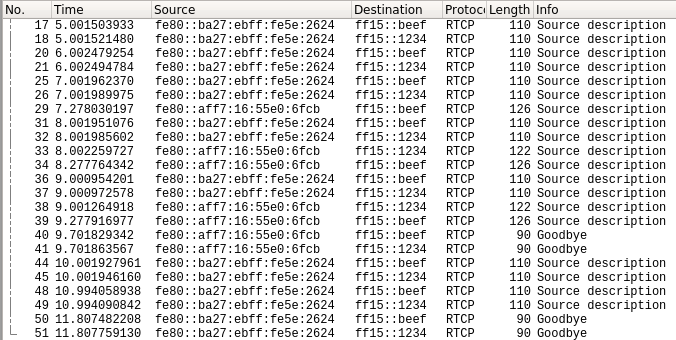
\includegraphics[width=\textwidth]{figures/wireshark_presence}
	\caption{Figure shows output from \program{Wireshark}. It should be noted, that until packet nr.26 is only fe80::ba27:.. sending RTCP SDES, but when \sub{} joins, it starts sending RTCP SDES to both the well known address ff15::beef and the source multicast group ff15::1234.} \label{fig:verify:wireshark_presence}
\end{figure}
From figure \ref{fig:verify:wireshark_presence} the RTCP SDES packets can be seen. Until packet no. 26 is only the \pub{} running. It can be seen that the \pub{} sends its RTCP SDES to both the well known multicast address(ff15::beef) and its source stream (ff15::1234). From packet nr.29, the \sub{} has been started, where it sends out an RTCP SDES to the well known multicast group. It has then joind the source multicast announced by the \pub{} from message no. 32, as the \sub{} sends RTCP SDES to the source stream too. From message no. 40 is the \sub{} gracefully shutting down as it sends a RTCP BYE to both source and well known multicast group. From message no. 50, the \pub{} is gracefully shutting down too.

Listing \ref{lst:verify:rtcpsdes} shows the ouput from a \sub{} receiving and parsing an RTCP SDES packet.

\begin{listing}[h] 
\begin{minted}{bash}
\$VAR1 = bless( {
                 'sdes' => {
                             '6c73c635' => {
                                             'LOC' => '',
                                             'PHONE' => '',
                                             'NAME' => '',
                                             'TOOL' => 'MCLURS',
                                             'NOTE' => '',
                                             'CNAME' => 'suas@batbox3',
                                             'EMAIL' => ''
                                           }
                           }
               }, 'Net::RTCP::Packet' );
\end{minted}
\caption{Listing shows part of the output from a \sub{} receiving and parsing an RTCP SDES packet sent by a \pub{}}
\label{lst:verify:rtcpsdes}
\end{listing}


\subsection{}

\begin{itemize}
	\item Tested with Lua/(post dissector) in wireshark. Transfer chunk of data of 4096 kb(page size) with counter in start of packet. Packet is read from wireshark and by writing dummy producer of 'X' x 4096.

	\item Show Byes are sent when publisher/subscriber are shutdown gracefully

	\item Show essential metadata are sent periodically as json/yml
	\item Show SDES \& BYE to both RTP sessions
	
\end{itemize}



\section{Verification} \label{sec:design:verification}
Several of the implementation requirements have been addressed in the chapter \ref{sec:implementation}. In order to verify the implementation and there by design works, 7 tests have been conducted.
\todo{Add what has not been fully implemented}

\todo{Describe in list which requirements are tested.}
\begin{itemize}
	\item \textbf{Session Announcement (Essential metadata)}\\
This test aims to verify the Session Announcement Mechanism with Essential metadata works as intended.
	\item \textbf{Presence Mechanism}\\
This test aims to verify the Presence Mechanism works as intended.
	\item IP collision resolver
This test aims to verify the \pub{} is able to generate a new multicast IP if there is a collision.
	\item Subscribe resolve MG
This test verifies the \sub{} can tage a session name, and resolve that into an multicast IP.
	\item Non-essential Metadata
This test verifies non-essential metadata can be sent and received.
	\item Record with tcpdump and replay with tcpreplay and see subscriber get same data.
This test verifies a stream can be recorded and replayed.
	\item Verify RTCP SR timestamps
This test is supposed to verify RTP SR timestamps are working, however at the moment of writing it does not work.
	\item Compare output from \con{} with output from \program{Snapshot}.
This verifies data sent from snapshot is the same as the \con{} receives.
\end{itemize}


\subsection{Session Announcement \& Essential metadata} \label{sec:verify:sessionannouncement}
This test verifies implementation requirement P8,P9 and S3. The goal of the test is to verify a SDP sent by a \pub{}, and verify a \sub{} can join an announced stream. \todo{add essential metdata tot}
The test has been conducted by staring a \pub{} that streams data from a \con{} which interfaces \program{Snapshot}. In order to verify the SDP is sent as an RTP packet, the traffic sent by the \pub{} has been inspected by \program{tcpdump}. Listing \ref{cmd:verify:sdp} shows the SDP packet sent by the \pub{}.

\begin{listing}[H] 
\begin{minted}{bash}
v=0
o=suas 3736400647 3736400647 IN IP4 batbox3
s=My Session
i=A fun session
u=http://www.ecs.soton.ac.uk/fun/
t=3736400647 3736404247
a=tool:publisher.pl uuid: E9A60146-618C
m=audio 5004 RTP/AVP 96
c=IN IP6 ff15::1234/5
a=quality:5
a=rtpmap:96 L16/220500/1
\end{minted}
\caption{SDP printed by the \pub{}}
\label{lst:verify:sdp}
\end{listing}

Figure \ref{lst:verify:tcpdumpsdp} shows the output from \program{tcpdump}.

\begin{listing}[H] 
	\begin{minted}{bash}
sudo tcpdump -i eth0 -X port 5004
11:04:08.895637 IP6 batbox3.local.5004 > ff15::beef.5004: UDP, length 270
        0x0000:  6006 4601 0116 110a fe80 0000 0000 0000  `.F.............
        0x0010:  ba27 ebff fe5e 2624 ff15 0000 0000 0000  .'...^&\$........
        0x0020:  0000 0000 0000 beef 138c 138c 0116 e83d  ...............=
        0x0030:  8000 0000 0001 e240 23e2 c753 763d 300a  .......@#..Sv=0.
        0x0040:  6f3d 7375 6173 2033 3733 3634 3030 3634  o=suas.373640064
        0x0050:  3720 3337 3336 3430 3036 3437 2049 4e20  7.3736400647.IN.
        0x0060:  4950 3420 6261 7462 6f78 330a 733d 4d79  IP4.batbox3.s=My
        0x0070:  2053 6573 7369 6f6e 0a69 3d41 2066 756e  .Session.i=A.fun
        0x0080:  2073 6573 7369 6f6e 0a75 3d68 7474 703a  .session.u=http:
        0x0090:  2f2f 7777 772e 6563 732e 736f 746f 6e2e  //www.ecs.soton.
        0x00a0:  6163 2e75 6b2f 6675 6e2f 0a74 3d33 3733  ac.uk/fun/.t=373
        0x00b0:  3634 3030 3634 3720 3337 3336 3430 3432  6400647.37364042
        0x00c0:  3437 0a61 3d74 6f6f 6c3a 7075 626c 6973  47.a=tool:publis
        0x00d0:  6865 722e 706c 2075 7569 643a 2045 3941  her.pl.uuid:.E9A
        0x00e0:  3630 3134 362d 3631 3843 0a6d 3d61 7564  60146-618C.m=aud
        0x00f0:  696f 2035 3030 3420 5254 502f 4156 5020  io.5004.RTP/AVP.
        0x0100:  3936 0a63 3d49 4e20 4950 3620 6666 3135  96.c=IN.IP6.ff15
        0x0110:  3a3a 3132 3334 2f35 0a61 3d71 7561 6c69  ::1234/5.a=quali
        0x0120:  7479 3a35 0a61 3d72 7470 6d61 703a 3936  ty:5.a=rtpmap:96
        0x0130:  204c 3136 2f32 3230 3530 302f 310a       .L16/220500/1.
	\end{minted}
\caption{The listing shows the output from \program{tcpdump}, listening on the well known multicast group. The bytes shown before the SDP packet is the ethernet header, UDP header and RTP header}
\label{lst:verify:tcpdumpsdp}
\end{listing}

It should be noted that the ASCII encoded content of the payload corresponds to the SDP packet in listing \ref{lst:verify:sdp}. Furthermore, a session is announce in the key starting with \textbf{C=IN...}.

In listing \ref{lst:verify:subsdp} is the output from a \sub{} shown, that receives the SDP.


\begin{listing}[h] 
\begin{minted}{bash}
SDP from 'publisher.pl uuid: E9A60146-618C', format: audio/L16/220500/1,\
	Multicast: ff15::1234:5004
Joining multicast group: ff15::1234:5004
<SDP printet>
Main-loop stopped with retval: NewRtp
Restarting loop due to new RTP stream joined
\end{minted}
\caption{Listing shows the output from a \sub{} that receives the SDP and joins the stream. It should be noted the event-loop is restarted, in order to also listen for the new multicast group}
\label{lst:verify:subsdp}
\end{listing}



\subsection{Presence Mechanism} \label{sec:verify:presencemechanism}
This test verifies implementation requirement P11-13 and S3. The goal of this test is to verify the presence mechanism works in both \sub{} and \pub{}. Due to lack of time, lists maintaining present participants have not been implemented, however RTCP SDES/BYE are sent and received by both \pub{} and \sub{}.
A test was conducted, where the \pub{} is started and some time later the \sub{} is started. The RTCP SDES sent by the \pub{} and \sub{} is shown in figure \ref{fig:verify:wireshark_presence}.

\begin{figure}[H]
	\centering
	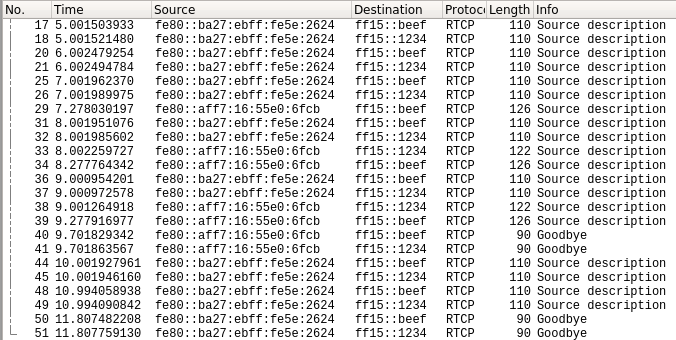
\includegraphics[width=\textwidth]{figures/wireshark_presence}
	\caption{Figure shows output from \program{Wireshark}. It should be noted, that until packet nr.26 is only fe80::ba27:.. sending RTCP SDES, but when \sub{} joins, it starts sending RTCP SDES to both the well known address ff15::beef and the source multicast group ff15::1234.} \label{fig:verify:wireshark_presence}
\end{figure}
From figure \ref{fig:verify:wireshark_presence} the RTCP SDES packets can be seen. Until packet no. 26 is only the \pub{} running. It can be seen that the \pub{} sends its RTCP SDES to both the well known multicast address(ff15::beef) and its source stream (ff15::1234). From packet nr.29, the \sub{} has been started, where it sends out an RTCP SDES to the well known multicast group. It has then joind the source multicast announced by the \pub{} from message no. 32, as the \sub{} sends RTCP SDES to the source stream too. From message no. 40 is the \sub{} gracefully shutting down as it sends a RTCP BYE to both source and well known multicast group. From message no. 50, the \pub{} is gracefully shutting down too.

Listing \ref{lst:verify:rtcpsdes} shows the ouput from a \sub{} receiving and parsing an RTCP SDES packet.

\begin{listing}[h] 
\begin{minted}{bash}
\$VAR1 = bless( {
                 'sdes' => {
                             '6c73c635' => {
                                             'LOC' => '',
                                             'PHONE' => '',
                                             'NAME' => '',
                                             'TOOL' => 'MCLURS',
                                             'NOTE' => '',
                                             'CNAME' => 'suas@batbox3',
                                             'EMAIL' => ''
                                           }
                           }
               }, 'Net::RTCP::Packet' );
\end{minted}
\caption{Listing shows part of the output from a \sub{} receiving and parsing an RTCP SDES packet sent by a \pub{}}
\label{lst:verify:rtcpsdes}
\end{listing}


\subsection{}

\begin{itemize}
	\item Tested with Lua/(post dissector) in wireshark. Transfer chunk of data of 4096 kb(page size) with counter in start of packet. Packet is read from wireshark and by writing dummy producer of 'X' x 4096.

	\item Show Byes are sent when publisher/subscriber are shutdown gracefully

	\item Show essential metadata are sent periodically as json/yml
	\item Show SDES \& BYE to both RTP sessions
	
\end{itemize}

\chapter{Discussion}\label{chp:discussion}
This chapter will discuss how the original limitations of MCLURS has been solved by the new design, and what new limitations has been imposed by the new architecture. The assumptions made for the new architecture will be discussed as well, and how they could be accommodated. At last, the functionality not implemented will be listed and discussed.

\subsection{MCLURS Limitations}

\noindent{}The MCLURS limitations from section \ref{sec:existingsystem:limitations} is summarized and listed below.
\begin{itemize}
	\item Bandwidth not fast enough on USB-bus to save locally and stream online
	\item Live processing not supported, as files are saved locally
	\item Responsibility not welldefined for RPi, as everything is running on the RPi
	\item Backup of recordings are not possible, as the recordings are only saved locally
\end{itemize} 

\myparagraph{Bandwidth}
Bandwidth has been solved, as an RPi is publishing its stream to a multicast group. This way bandwidth is only used to capture samples from the USBDUX-fast, and send it to the ethernet interface.
 
\myparagraph{Live Processing}
Live processing of recordings is possible in the new architecture, as the recordings are available on a multicast group. A \sub{} can be told to subscribe to a stream, in order to process the stream live. As there is no requirement for how long a time it must take for a sample captured by the ADC to be available on a multicast group, this has not been investigated further. This could be tested by making a high frequency sound and seeing how long time it takes from the sound being generated to the sound being received by a \program{filter} on the network.

\myparagraph{Responsibility}
The responsibility of a RPi is more well-defined in the new architecture as the RPi is just responsible for capturing samples, and streaming them to multicast. It is up to other nodes on the network to save or process the stream.

\myparagraph{Backup of Recordings}
The \hist{} is designed to be the node responsible for saving recordings to local storage. As all streams are available on multicast groups, multiple \program{Historians} can be connected to the network. This allows multiple \program{Historians} to save the streams to multiple disks simultaneously, and thereby creating a backup. However both \program{Historians} will save the same data, so if packets are lost during transmission, depending on where the packet is lost, both \program{Historians} will miss the packet.\\

\subsection{Assumptions}
\noindent{}In the beginning of the analysis, some assumptions were made in order to limit the scope of the project. These assumptions are summarized and listed below.
\begin{itemize}
	\item No packet loss or corruption during transmission
	\item No bandwidth limitation
	\item No security is taken into consideration
\end{itemize}

No packet loss should be a reasonable assumption on small networks; However, if the application cannot risk losing packets, different protocols should be taken into consideration.
One such protocols could be \ac{PGM}\footnote{\url{https://en.wikipedia.org/wiki/Pragmatic\_General\_Multicast}} which is a protocol developed in order to reliably deliver packets to all multicast participants.
PGM works by sending NAKs from a receiving participant when a packet is lost, unicast back to the sender or a designed participant on the network(Designated Local Repairer(DLR)), responsible for resending packets. A NAK confirmation(NCF) is sent back unicast to the receiving participant, such that it knows the NAK it emitted has been received. The sender or DLR will then unicast resend the missing packet to the participant sending the NAK. PGM is not implemented in Linux; However, openpgm\footnote{\url{https://code.google.com/archive/p/openpgm/}} is a library that implements PGM.\\

\noindent{}No bandwidth limitation is also a reasonable assumption is small systems, however as each RPi consumes 48 Mbits/s, the network can consist of a maximum of 20 RPis if a 1 Gbit/s switch is used. The switch(s) used might pose a limitation on the number of packets it can handle, but this should not be an issue since the RTP packets are relatively large.  If a limitation arises on the port in the switch where the \hist{} is connected, as the port on the 1 Gbit/s switch is not capable of providing more than 1 Gbit/s of data, to mitigate this two \program{Historian} can be used, each only saving half of the streams. This might, however, pose new complexity of synchronizing replay of the two \program{Historians}. Instead a 10 Gbit/s switch could be used which would raise the limit to approximately 200 RPis producing data on the network.\\

\noindent{}No security is taken into consideration but, as mentioned in section \ref{sec:design:profile}, profiles for encrypting RTP packets exist and could be used.

\subsection{Implementation Details}

The way a \pub{} and a \sub{} run a \pro{} and \con{} respectively, is similar to how Daniel Bernstein has implemented his \textit{ucspi-tcp}. \textit{ucspi-tcp} is a suite of tools for running a tcpserver, tcpclient etc. The tcpserver takes a program as argument, which is invoked for each connection handled by tcpserver. Relevant information about the client is then passed as arguments to the program. This is especially used in  \program{qmail}, where \textit{tcpserver} creates a listening socket on port 25, and runs \textit{qmail-smtpd} for each connection.\footnote{\url{http://cr.yp.to/ucspi-tcp.html}}. Running programs this way provides great modularity in the way programs can be run and connected using e.g. pipes. The price of running \pros{} and \cons{} this way is, that the \sub{} and \pub{} should implement error handling in case a \con{} or \pro{} crashes. This is especially true when a \program{Filter} is run by a \pub{} which is run by a \sub{}, and the \program{Filter} suddenly dies. The \pub{} should then report the error, stop and die gracefully followed by the \sub{} doing the same. As mention in section \ref{sec:existingsystem:software}, MCLURS is run under supervison from runit. Runit could also be used to run the \sub{} and \pub{}. 


\noindent{}As stated in a footnote in section \ref{sec:design:presencemechanism}, it is known a race condition might occur if two \pubs{} join a stream at the same time. A solution would be to use an algorithm inspired by e.g. \ac{DHCP} such that a message is sent to the well known multicast group, where the \pub{} asks if any has the address it's about to use. If nobody replies, the multicast group should be free.


\noindent{}Due to lack of time, several features have not been fully implemented.
Those features are listed below:
\begin{itemize}
	\item Essential metadata is not passed through the metadata pipe to the \con{}.
	\item Events have not been tested. As events are sent over an RTP stream as samples(which is known to work), events SHOULD\footnote{It is known by the author that things doesn't necessarily work even though they should} also work.
	\item YML is not implemented, only JSON.
	\item Participant-lists are not implemented in the \sub{} and \pub{} for the presence mechanism.
	\item RTCP SR timing is not correct, as explained in section \ref{sec:verify:rtcpsr}.
	\item When running the \sub{} starting the \pub{} starting the \program{Filter}, the SSRC from the RTP packets should be passed to the \pub{} such that the \pub{} can add the SSRC to the CSRC list. 
	\item Continuous submission of snapshots has not been implemented. When the initial count of snapshots have finished, snapshot will stop writing data and close the pipe.
	\item Running a filter by letting the \sub{} run the \pub{} which starts the \program{Filter}.
	\item If the \program{filter} requires a specific chunk size, it would be sensible to add a parameter to the \sub{} that says how large a chunks of data should be written to pipe between the \sub{} and the \program{Filter}. This requires a buffer in the \sub{} to be implemented.
\end{itemize}

The \pub{} and \sub{} should be implemented in C, in order to provide language bindings for other languages, such that the \pub{} and \sub{} can be used in different implementations.




\chapter{Conclusion}
The existing recording system, MCLURS, has been redesigned such MCLURS can be used in new use cases requiring online processing and monitoring of recordings. Instead of saving recordings to files locally on each RPI, the new design utilizes multicast groups to distribute streams among those network nodes that want particular streams. From the Analysis a list of requirements where extracted and mapped into widely-used streaming protocols with success. Four software components have been introduced that follow from design requirements, are modular by design, and thereby make it relatively easy to interface MCLURS to the streams. The design has been tested by making proof-of-concept implementations written in PERL which, using a C RTP library make it possible to send streams of samples over a multicast group. This stream can then be received again and tested to be the exact same as the stream of samples that was sent. Mechanisms were implemented that take care of multicast group collisions; however, it turned out to be susceptible to deadlocks. A designated network node named a \hist{} has been defined to be responsible for recording and replaying streams. From a test, it was shown that the \hist{} is perfectly capable of recording streams and replaying them again without losing or changing the order of packets. \\

\noindent{}As mentioned in chapter \ref{chp:discussion}, not all requirements have been successfully verified and some functionality has not been implemented, due to lack of time. Performance testing of the implementation has not been done either; However these results will be presented at exam\\

\noindent{} Overall the suggested architecture has proved to fulfill the requirements extracted from the use cases, but more time should be spent pushing the suggested architecture to its limits.\\

\noindent{}For the future aspect of the project, the list from the Discussion of features not fully implemented would be a good place to start. An EventHistorian could be implemented that allows, the user to search through the events. If collected events are events saying when a bat is present, it could be useful to the biologist to be able to query the EventHistorian to get a list of e.g. the average number of bats during night-time. As the events are hierarchical key/value pairs, a NoSQL database could be used to store the event. Most NoSQL databases take JSON-encoded data as input meaning the events could be put directly into the NoSQL database. As  there is no inherent relation between events and anything else, there is no immediate need for a relational database.\\

\noindent{}The code developed for this project can be found at \url{https://github.com/Exchizz/master}

\chapter{Futore Work}


\appendix
\chapter{Deploy with Ansible}
Ansible stuff

\include{sections/appendex_array-cmd-flowchart}


\bibliographystyle{plain}
\bibliography{mybib}
\listoftodos
\end{document}